% !TEX encoding = UTF-8 Unicode
% -*- coding: UTF-8; -*-
% vim: set fenc=utf-8

% true = makes the whole document (except images) black and white, to make the document suitable for printing
\newif\ifprint\printtrue

% use coppetex style class
\documentclass[grad,numbers,final]{coppetex/coppe}

% https://tex.stackexchange.com/questions/331430/produce-a-monochrome-pure-black-and-white-pdf-using-xelatex
\ifprint
\usepackage[monochrome]{xcolor}
\fi

\usepackage{iftex}
% https://tex.stackexchange.com/questions/47576/combining-ifxetex-and-ifluatex-with-the-logical-or-operation
\newif\ifxetexorluatex
\ifxetex
  \xetexorluatextrue
\else
  \ifluatex
    \xetexorluatextrue
  \else
    \xetexorluatexfalse
  \fi
\fi

\ifPDFTeX
  % use UTF-8 in pdftex (not needed in LuaTeX and XeTeX)
  \usepackage[utf8]{inputenc}
\fi

% math and symbols
\usepackage{amsmath,amssymb}

 % next-gen computer modern fonts
\usepackage{lmodern}

% better placement of images in subsections
\usepackage[section]{placeins}

% https://en.wikibooks.org/wiki/LaTeX/Floats,_Figures_and_Captions
\usepackage{float}

% figures with borders
\floatstyle{boxed}
\restylefloat{figure}

% required for better figures
\usepackage{subfigure}

% required for better tables
\usepackage{longtable}
\usepackage{multirow}
\usepackage{makecell}

% curly brackets besides tables (\ldelim, \rdelim)
\usepackage{bigdelim}

% quotes
\usepackage{epigraph}
\setlength{\epigraphrule}{0pt}

% text highlighting, underlining, spacing
\usepackage{soul}

% todo notes
\usepackage[obeyFinal,portuguese,colorinlistoftodos,textsize=footnotesize]{todonotes}
\newcommand{\mattoso}[2][]{\sethlcolor{pink}\texthl{#1}\todo[author=\textbf{Marta Mattoso},inline,color=pink]{#2}}
\newcommand{\perrotta}[2][]{\sethlcolor{orange}\texthl{#1}\todo[author=\textbf{Thiago Perrotta},inline,color=orange]{#2}}
\newcommand{\silva}[2][]{\sethlcolor{lightgray}\texthl{#1}\todo[author=\textbf{Vitor Silva},inline,color=lightgray]{#2}}

% captions for floats
\usepackage[labelfont=bf]{caption}

% source code listings
\usepackage{listings}

% https://www.overleaf.com/help/193-what-otf-slash-ttf-fonts-are-supported-via-fontspec
% https://www.overleaf.com/help/73-i-have-a-custom-font-id-like-to-load-to-my-document-how-can-i-do-this
\ifxetexorluatex
  \usepackage{fontspec}
  \newfontfamily{\lstsansserif}[Scale=.80]{Fira Mono}
  \lstset{basicstyle=\lstsansserif}
\else
  \lstset{basicstyle=\footnotesize\sf}
\fi

\lstset{%
  aboveskip=15pt,
  belowskip=15pt,
  breakatwhitespace=false,     % sets if automatic breaks should only happen at whitespace
  breaklines=true,             % sets automatic line breaking
  postbreak=\mbox{\textcolor{red}{$\hookrightarrow$}\space},
  captionpos=t,                % sets the caption-position
  columns=fullflexible,
  commentstyle=\color{gray},   % sets the comments color
  escapechar=\%,               % write LaTeX inside listings
  frame=lines,                 % adds a frame
  numbers=left,                % where to put the line-numbers
  numberstyle=\footnotesize\color{gray}, % the size of the fonts that are used for the line-numbers (alt: \tiny)
  showspaces=false,            % show spaces adding particular underscores
  showstringspaces=false,      % underline spaces within strings
  showtabs=false,              % show tabs within strings adding particular underscores
  stepnumber=1,                % the step between two line-numbers. If it's 1 each line
  stringstyle=\color{gray},
  tabsize=2,                   % sets default tabsize to 4 spaces
  title=\lstname,              % show the filename of files included with \lstinputlisting;
}

\lstdefinelanguage{sqlresults}{%
  aboveskip=5pt,
  belowskip=5pt,
  basicstyle=\footnotesize\ttfamily,
  columns=fixed,
  numbers=none,
  frame=none,
}

% highlight the following keywords for pseudocode listings
% \lstdefinelanguage{pseudocodigo}{%
\lstdefinelanguage{pseudocode}{%
    % morekeywords={se,então,para,cada,faça,fim,função,retorna,enquanto,não,is,ou,e,senão,novo,termina,continua,verdadeiro,falso},
    morekeywords={if,then,for,each,do,end,function,return,while,not,is,or,and,else,new,break,continue,true,false},
    sensitive=true, % case-sensitive keywords?
    morecomment=[l]{\#}, % comments are lines that start with a #
}

% display list of figures, tables or listings only if at least one component is present
\usepackage[figure,table,lstlisting]{totalcount}

% hyperlinks
\usepackage{hyperref}

\ifprint
\hypersetup{%
  portuguese,
  pdfencoding=auto,
  breaklinks=true,
  bookmarksopen=true,
  colorlinks=false,
  hidelinks,
  pdfborder={0 0 0},
}
\else
\hypersetup{%
  portuguese,
  pdfencoding=auto,
  breaklinks=true,
  bookmarksopen=true,
  colorlinks=true,
}
\fi

\makelosymbols{}
\makeloabbreviations{}

% include only the following chapters (faster typesetting)
% \includeonly{%
%  chapter01,
% }

\begin{document}
  \title{Análise do Rastro de Proveniência em Simulações Computacionais em Larga Escala}
  \foreigntitle{Provenance Tracing Analysis on Large-Scale Computer Simulations}

  \author{Thiago}{Barroso Perrotta}
  % http://www.cos.ufrj.br/~marta/
  \advisor{Profa.}{Marta}{Lima de Queirós Mattoso}{D.Sc.}
  % http://www3.cos.ufrj.br/index.php?option=com_pescstaff&Itemid=110&func=fullview&staffid=2276
  \advisor{}{Vítor}{Silva Sousa}{M.Sc.}

  % http://www.cos.ufrj.br/~marta/
  \examiner{Profa.}{Marta Lima de Queirós Mattoso}{D.Sc.}
  % http://www3.cos.ufrj.br/index.php?option=com_pescstaff&Itemid=110&func=fullview&staffid=2276
  \examiner{}{Vítor Silva Sousa}{M.Sc.}
  % http://www.cos.ufrj.br/~assis/
  \examiner{Prof.}{Alexandre de Assis Bento Lima}{D.Sc.}
  % https://renan-souza.github.io/
  \examiner{}{Renan Francisco Santos Souza}{M.Sc.}

  \department{PESC}

  \date{09}{2017}

  \keyword{\textit{Workflows} Científicos}
  \keyword{Análise de Dados Científicos}
  \keyword{Gerência de Fluxos de Dados}
  \keyword{Dados de Proveniência}
  \keyword{Bancos de Dados}

  \foreignkeyword{Scientific Workflows}
  \foreignkeyword{Raw Data Analysis}
  \foreignkeyword{Dataflow Management}
  \foreignkeyword{Provenance Data}
  \foreignkeyword{Databases}

  \listoftodos{}

  \maketitle
  \frontmatter{}

  % !TEX encoding = UTF-8 Unicode
% -*- coding: UTF-8; -*-
% vim: set fenc=utf-8

\dedication{Dedico esse trabalho aos meus pais.}

\chapter*{Agradecimentos}

Agradeço a minha mãe e ao meu pai, por todo o carinho e apoio que recebi, por serem meu exemplo de vida, e por sempre permanecerem presentes ao meu lado, tanto nas fases boas quanto nas ruins.

Agradeço ao Vítor Silva e à professora Marta Mattoso, meus orientadores, por todo o inestimável suporte e atenção nas diversas reuniões de projeto que tivemos, essenciais para o êxito desse trabalho.

Agradeço à professora Márcia Cerioli e ao professor Ricardo Marroquim, pela orientação durante meu período de iniciação científica na UFRJ.

Agradeço ao meu amigo Bruno Buss pelo voto de confiança.

Agradeço ao meu \textit{ex-host} na Google, Andy Venikov, por toda a liderança e motivação.

Também agradeço ao Donald Knuth e ao Leslie Lamport, por tornarem agradável a composição desse trabalho através do \TeX{} e do \LaTeX{}, respectivamente.

Por fim, agradeço aos meus bons amigos, os quais dia a dia fazem-me crescer e tornar-me uma pessoa cada vez melhor, e à serendipidade da vida.

\begin{center}
	\so{Muito obrigado a todos vocês!}
\end{center}

\vfill{}

% https://tex.stackexchange.com/questions/53377/inspirational-quote-at-start-of-chapter
\epigraph{\textit{``Really pay attention to negative feedback and solicit it, particularly from friends\ldots{} hardly anyone does that, and it's incredibly helpful.''}}{--- \textsc{Elon Musk}}


  % !TEX encoding = UTF-8 Unicode
% -*- coding: UTF-8; -*-
% vim: set fenc=utf-8

\begin{abstract}

Simulações computacionais frequentemente consomem e produzem grandes volumes de dados, parte dos quais é armazenada em arquivos brutos em %silva2015analyzing
diversos formatos de acordo com o domínio da aplicação, %silva2017raw
tal como o \textit{HDF5} em simulações de dinâmica de fluidos computacionais. %silva2017raw
Durante essas simulações, usuários em geral precisam rastrear grandezas de interesse (como resíduos e estimativas de erros) %silva2016situ % +tempo de execução
com base em elementos de dados relacionados de vários arquivos, a fim de controlar sua execução ao máximo possível. %silva2016situ
No entanto, esse rastreio costuma ser feito somente ao fim da simulação. %silva2016situ
Apesar dos formatos de arquivo serem apoiados por diversas linguagens de programação e bibliotecas,
os usuários comumente precisam desenvolver programas \textit{ad-hoc} para realizarem uma análise em grande escala, %silva2015analyzing
a qual pode ser ainda mais custosa se realizada com bancos de dados, pois eles exigem que os dados científicos sejam estruturados e carregados em memória. %silva2015analyzing
Nesse cenário, Sistemas de Gerência de Workflows Científicos (\textit{SGWfC}) com ciência do fluxo de dados têm empregado a abstração de \textit{workflows} científicos para apoiar a execução paralela dessas simulações, em que os dados de proveniência podem favorecer a gerência de elementos de dados relacionados em múltiplos arquivos de dados científicos (\textit{i.e.}, produzidos por diferentes programas de simulação). %silva2015analyzing
Esse trabalho utiliza a arquitetura de componentes ARMFUL, que baseia-se em dados de proveniência para extrair e
relacionar grandezas de interesse; mais especificamente, contribui com um mecanismo de processamento de consultas durante a execução de simulações computacionais, considerando-se o fluxo de elementos de dados ao longo das mesmas. %vitor

\end{abstract}

\begin{foreignabstract}

Computer simulations frequently consume and produce lots of raw data files, which usually follow a \textit{de facto} standard data format established by the application domain, such as \textit{HDF5} in fluid dynamics simulations.
In these simulations, users often need to track quantities of interest (such as residuals and error estimates) based on elements of related data from several raw files, in order to control as much as possible its execution.
Nonethless, this tracking is usually done only once the simulation ends.
Notwithstanding the file formats being supported by several programming languages and libraries, users generally need to develop ad-hoc programs to perform a specific analysis in large scale, which can be even more costly if performed with databases, because they require the raw data files to be structured and loaded in memory.
In this scenario, dataflow-aware Scientific Workflow Management Systems (SWfMS) have resorted % alt: employed
to scientific workflow abstractions to support parallel execution of these simulations, in which provenance data can help to manage related data files in multiple raw data files (\textit{i.e.}, produced by different simulation programs).
This work uses the component-based ARMFUL architecture, which is based on provenance data to extract and relate quantities of interest; more precisely, it contributes with a query processing mechanism for computer simulations, considering the flow of data elements during its execution.

\end{foreignabstract}


  \tableofcontents
  
  \iftotalfigures
  \listoffigures
  \fi
  
  \iftotaltables
  \listoftables
  \fi
  
  \iftotallstlistings
  \renewcommand{\lstlistlistingname}{Lista de Códigos}
  \renewcommand{\lstlistingname}{Código}
  \clearpage
  \addcontentsline{toc}{chapter}{\lstlistlistingname}
  \lstlistoflistings{}
  \fi

  \printloabbreviations{}
  \printlosymbols{}

  \mainmatter{}
  % !TEX encoding = UTF-8 Unicode
% -*- coding: UTF-8; -*-
% vim: set fenc=utf-8

\chapter{Introdução}

Neste capítulo são apresentadas a visão geral e a motivação desta monografia, além da contribuição proposta.

\section{Visão geral e Contextualização}

% Simulações computacionais...análises...hipóteses científicas...
Simulações computacionais tornaram-se predominantes e omnipresentes no dia-a-dia de cientistas\footnote{Daqui em diante denominados \textit{usuários}.}, sendo necessárias na realização de análises que utilizam modelos computacionais complexos que lidam com grandes volumes de dados~\cite{silva2015analyzing}. Isso permite a exploração de dados específicos de domínio para apoiar esses usuários na validação de hipóteses científicas ou comportamentos peculiares.

% Muitos programas...consumem e produzem muitos dados...
Essas simulações geralmente envolvem a execução de muitos programas do domínio científico, os quais intensivamente consomem e produzem muitos dados. A maior parte desses dados é armazenada em diversos formatos de arquivo também no domínio da aplicação~\cite{silva2015analyzing}, por exemplo, \abbrev{FITS}{Flexible Image Transport System} FITS~\cite{greisen2002representations} em astronomia, ou \abbrev{HDF}{Hierarchical Data Format} HDF5~\cite{folk1999hdf5} e \abbrev{NetCDF}{Network Common Data Form} NetCDF~\cite{rew1990netcdf} em dinâmica de fluidos computacionais.
% Longo tempo para ser executada...mesmo em PAD...
Uma grande parte dessas simulações computacionais em larga escala leva um longo tempo para ser executada, mesmo em ambientes de \abbrev{PAD}{Processamento em Alto Desempenho} PAD (Processamento em Alto Desempenho)~\cite{silva2017raw}, onde o poder de computação é amplificado através da utilização de diversos núcleos computacionais.

% Rastrear grandezas...somente no fim...programas ad-hoc...SGBD...
Durante as simulações, usuários com frequência precisam rastrear grandezas de interesse, tais como resíduos, tempo de execução e estimativas de erro, baseadas em elementos de dados relacionados de vários arquivos, a fim de controlar a sua execução ao máximo possível~\cite{silva2016situ}. Contudo, esse rastreamento costuma ser realizado manualmente durante a execução dessas simulações. Nesse caso, a alternativa torna-se realizar esse rastreamento somente ao fim das simulações, o que não é prático para o usuário, já que essas simulações levam um tempo considerável de execução mesmo em PAD~\cite{silva2017raw}. Além disso, mesmo considerando que os arquivos produzidos sejam tipicamente apoiados por diversas linguagens de programação e bibliotecas, diversos programas \textit{ad-hoc} precisam ser desenvolvidos a fim de permitir análises em grande escala.

% MARTA: remover essa parte:
% , as quais se tornam ainda mais custosas se realizadas com \abbrev{SGBD}{Sistema de Gerenciamento de Banco de Dados} SGBDs (Sistemas de Gerenciamento de Banco de Dados), pois eles aumentam a complexidade de execução em termos da estruturação e da carga dos dados ~\cite{silva2015analyzing}.

\section{Motivação}%
\label{sec:motivacao}

% SGWfCs...paralelização...proveniência...
As simulações computacionais podem ser gerenciadas por um \abbrev{SGWfC}{Sistema de Gerência de \textit{Workflows} Científicos} SGWfC (Sistema de Gerência de \textit{Workflows} Científicos) paralelo, tal como o Kepler~\cite{ludascher2006scientific} e o Pegasus~\cite{deelman2005pegasus}, o que faz com que se beneficiem da proveniência e do paralelismo de dados entre os diferentes programas que compõem o seu \textit{workflow}\footnote{Em tradução livre, ``fluxo de trabalho''. No entanto, daqui em diante continuaremos a utilizar \textit{workflow}, por ser um termo mais preciso.}~\cite{bux2013parallelization}.
% Workflows...dataflows(dt, ds, phi)...DAG...
Tais \textit{workflows} científicos são composições de tarefas de processamento de dados sequenciais e concorrentes, cuja ordem de execução é determinada com base nas interdependências entre os dados~\cite{bux2013parallelization}. Eles podem ser modelados através de um fluxo de dados (\textit{dataflow}) que descreve todos os conjuntos de dados, atributos de dados, transformações de dados e dependências entre os mesmos~\cite{silva2017raw}. Esses fluxos de dados são usualmente especificados na forma de um \abbrev{DAG}{Directed Acyclic Graph --- Grafo Direcionado Acíclico} DAG (grafo direcionado acíclico), em que transformações de dados são representadas como nós, e conjuntos de dados são modelados como arestas direcionadas.

% Trade-offs entre usabilidade e poder de controle...
Os SGWfCs são usualmente difíceis de serem configurados e utilizados pelos usuários -- alguns deles, tais como o Taverna~\cite{hull2006taverna}, possuem uma boa ênfase em usabilidade, porém não compensam na paralelização e utilização de recursos computacionais distribuídos, perdendo, assim, sua efetividade.
% Dificuldade em não utilizar SGWfCs...
Eles facilitam o \textit{design}, a manutenção, a execução e o monitoramento de \textit{workflows} científicos. Entretanto, sem suporte ao rastreamento de dados científicos, o desafio é analisar a propagação de dados de conjuntos de arquivos ao longo da execução da simulação, o que é bastante propenso a erros se realizado manualmente~\cite{silva2015analyzing}. Isso porque são necessários: \( (i) \) a nomenclatura de arquivos de forma apropriada; \( (ii) \) escrever e gerenciar programas \textit{ad-hoc} para gerenciar cada transformação de dados e arquivos; e \( (iii) \) mapear o fluxo das transformações de dados, assim como dos elementos de dados consumidos e produzidos pela execução de cada transformação de dados.

% Marta(antes): Existem três tipos básicos de consultas\footnote{Isso será mais aprofundado no~\autoref{chap:analise-solucoes-consultas-dados-cientificos}.} que são rotineiramente utilizadas em simulações científicas:

Silva et al.~\cite{silva2015analyzing} consideram que existem três tipos básicos de consulta\footnote{Isso será mais aprofundado no~\autoref{chap:analise-solucoes-consultas-dados-cientificos}.} que são rotineiramente utilizadas em simulações científicas:

\begin{enumerate}
    \item conteúdo de arquivo específico de domínio;
    \item múltiplos arquivos relacionados através de transformações de dados / programas de simulação; e
    \item elementos de dados relacionados de múltiplos arquivos
\end{enumerate}

% Por exemplo, o FastBit~\cite{wu2009fastbit} é capaz de realizar apenas consultas do tipo 1, o Chiron~\cite{ogasawara2013chiron} é capaz de realizar consultas dos tipos 1 e 2, enquanto o NoWorkflow~\cite{murta2014noworkflow} e o Tigres~\cite{hendrix2016tigres} são capazes de realizar consultas dos tipos 2 e 3. Contudo, os dois últimos não são focados em dados científicos presentes em arquivos.

\section{Contribuição}

% Desse modo, como vimos na última seção, a capacidade de realizar todos os três tipos de consultas citados ainda é um problema em aberto, sendo especialmente importante em situações de larga escala, onde muitos dados são manipulados intensivamente.
Silva et al.~\cite{silva2015analyzing} observam que a capacidade de realizar todos os três tipos de consultas citados ainda é um problema em aberto, sendo especialmente importante em situações de larga escala, onde muitos dados são manipulados intensivamente.
Para preencher esse gargalo, Silva et al.~\cite{silva2015analyzing} propuseram a arquitetura \abbrev{ARMFUL}{Analysis of Raw Data from Multiple Files} ARMFUL (Analysis of Raw Data from Multiple Files)~\cite{silva2017raw,silva2016situ}: com ela, todos os três tipos de consultas podem ser realizados. Todos esses tipos de consultas podem ser apoiadas pela ARMFUL ao oferecer uma base de dados de proveniência, cujo objetivo é guardar as referências para os arquivos e os elementos de dados do domínio da aplicação selecionados pelos usuários, para que eles possam ser devidamente rastreados~\cite{silva2015analyzing}.

Dessa forma, os usuários podem submeter consultas para selecionar dados científicos de suas simulações não apenas após, mas também durante a execução da simulação: o objetivo é a possibilidade de captação dos elementos de dados de interesse no momento em que eles são gerados~\cite{silva2015analyzing}. O benefício dessa abordagem é evitar que a extração (\textit{parsing}) dos dados tenha que ocorrer por completo, em vez disso, ela pode ser realizada dinamicamente (\textit{on-the-fly}), sem ter que fazer todo o carregamento dos dados em memória ou em um SGBD (Sistema de Gerenciamento de Banco de Dados) \abbrev{SGBD}{Sistema de Gerenciamento de Banco de Dados}, o que evita a duplicação e a manutenção de dados no SGBD, e também reduz o custo computacional da consulta, que passa a ser realizada em menos tempo.

% MARTA: essa é a definição do meu problema.
Apesar da arquitetura ARMFUL ser bem abrangente e eficiente em prover consultas envolvendo dados de domínio, de proveniência e de execução, ela oferece um recurso limitado para o usuário submeter consultas dessas três classes. Na verdade, o usuário precisa não apenas conhecer bem a linguagem SQL, mas também os relacionamentos necessários para permitir o rastreamento entre múltiplos arquivos de dados.
Este trabalho tem por objetivo facilitar essa interação do usuário com a elaboração de consultas analíticas ao utilizar a ARMFUL.

Mais especificamente, a contribuição deste trabalho é uma extensão da arquitetura ARMFUL apresentada em~\cite{silva2016situ,silva2017raw} com a introdução de um processador de consultas, denominado QPP (\textit{Query Preprocessor}) \abbrev{QPP}{Query Preprocessor --- Pré-Processador de Consultas}. O QPP atua como um componente do ARMFUL que é responsável pela interação do usuário com os conjuntos de dados de suas simulações. A partir dele, o usuário é capaz de escrever uma consulta sem ter que aprender \abbrev{SQL}{Structured Query Language} SQL (\textit{Structured Query Language}), pois ela é representada em alto nível, em um formato que é posteriormente traduzido (convertido) para SQL de forma transparente para o usuário. Isso pode facilitar o uso do sistema, já que o usuário não precisaria ter profundos conhecimentos em SQL e poderia se preocupar apenas com o domínio da aplicação da simulação computacional e com os dados e grandezas de interesse para as consultas.
% REMOVER(Renan): O benefício imediato disso é diminuir a curva de aprendizado para que uma consulta possa ser realizada, pois o usuário precisa se preocupar \textit{a priori} apenas com o domínio da aplicação da simulação computacional e com os dados e grandezas de interesse que ele deseja consultar.

Outro benefício é o desempenho atingido com as consultas: o QPP faz o pré-processamento da especificação da simulação computacional --- que só precisa ser realizado uma única vez, sempre que o QPP é executado durante uma sessão --- em estruturas de dados eficientes em relação aos dados obtidos pelo componente de Captura de Dados de Proveniência (ou, do termo em inglês, \textit{Provenance Gatherer}) da arquitetura ARMFUL. Desse modo, consultas consecutivas beneficiam-se da proveniência já carregada na memória; reduzindo, portanto, o tempo de processamento.

\section{Estruturação do Texto}

A principal contribuição deste trabalho consiste no desenvolvimento do QPP: como ele foi criado, como ele se integra à arquitetura ARMFUL previamente apresentada, e quais são os benefícios --- qualitativamente e quantitativamente --- que ele acrescenta à mesma.

Assim, ele está organizado da seguinte forma:
o \autoref{chap:referencial-teorico} apresenta o embasamento teórico, introduzindo e definindo os conceitos, definições e a terminologia que será utilizada ao longo do trabalho.
No \autoref{chap:analise-solucoes-consultas-dados-cientificos} listamos algumas publicações relacionadas e recentes, algumas dentre as quais serviram como motivação e base para essa, e também abordamos a diferença entre os tipos de consulta mais comuns em simulações científicas.
O \autoref{chap:arquitetura-armful} aborda a arquitetura ARMFUL e apresenta o \textit{DfAnalyzer}.
No \autoref{chap:rastros-de-proveniencia} desenvolvemos a abordagem e mostramos os algoritmos utilizados para analisar rastros de proveniência dos arquivos e dados científicos de simulações computacionais.
No \autoref{chap:experimentos} são abordados os resultados obtidos através do QPP e os experimentos realizados com o mesmo.
Finalmente, o \autoref{chap:conclusao} conclui o trabalho com perspectivas de trabalhos futuros.
 % Introduction
  % !TEX encoding = UTF-8 Unicode
% -*- coding: UTF-8; -*-
% vim: set fenc=utf-8

% REVIEW: {referencial, embasamento} teórico
\chapter{Referencial Teórico}%
\label{chap:referencial-teorico}

\perrotta{Capítulo 02 --- Referencial Teórico}

Nessa seção serão abordados alguns conceitos e a terminologia que será utilizada ao longo desse trabalho.

\section{Simulação Computacional}

\section{Dataflow}

Uma especificação de fluxo de dados \( D_F \) é definida como \[ D_F = (T, S, \Phi) \] onde:
\begin{itemize}
    \item \( T = \{t_1, t_2, \ldots, t_{\alpha}\} \) \vdots{}
    \( \{t_i \mid i \in \{{1, 2, \ldots, \alpha}\} \} \)
    é transformação
    \item \( S = \{s_1, s_2, \ldots, t_{\beta}\} \) \vdots{}
    \( \{s_i \mid i \in \{{1, 2, \ldots, \beta}\} \} \)
    é conjunto de dados
    \item \( \Phi = \{\phi_1, \phi_2, \ldots, \phi_{\gamma}\} \) \vdots{}
    \( \{\phi_i \mid i \in \{{1, 2, \ldots, \gamma}\} \} \){}
    é dependência de dados
\end{itemize}

\missingfigure{Exemplo de -> o ->, i.e., transformação com dataset de entrada e de saída}

\perrotta{Acho que falta definir o que é uma transformação.}

\subsection{Dependência de dados}

Uma especificação de dependência de dados \( \phi \) é definida como \[ \phi = (s, t_{\textrm{previous}}, t_{\textrm{next}}) \] onde:
\begin{itemize}
    \item \( s \) é um conjunto de dados
    \item \( t_{\textup{previous}} \) é a transformação que {\bf produz} dados para o conjunto de dados \( s \)
    \item \( t_{\textup{next}} \) é a transformação que {\bf consome} dados do conjunto de dados \( s \)
\end{itemize}

\subsection{Conjunto de dados}

A especificação de um conjunto de dados \( s \) é dada por \[ s = (A, C) \] onde:
\begin{itemize}
    \item \( A = \{a_1, a_2, \ldots, a_{\delta} \} \; \vdots{} \; \{ a_i \mid i \in \{1, 2, \ldots, \delta \} \} \) é atributo
    \item \( C = \{c_1, c_2, \ldots, c_{\zeta} \} \; \vdots{} \; \{ c_i \mid i \in \{1, 2, \ldots, \zeta \} \} \) é coleção de dados
\end{itemize}

\subsection{Atributo}

Um atributo é especificado da seguinte forma: \[ a = (\textrm{nome},\textrm{tipo}) \therefore \textrm{tipo} = \{\textup{inteiro}, \textup{ponto flutuante}, \textup{texto}, \textup{arquivo}\} \]

\subsection{Coleção de dados}

Uma coleção de dados é definida como \[ c = \{ i_1, i_2, \ldots, i_{\eta} \} \; \vdots \; \{ i_j \mid j \in \{ 1, 2, \ldots, \eta \} \} \] é item de dados

\subsection{Item de dados}

A especificação de um item de dados é dada por \[ i = (s, T^{\ast}_{\textrm{previous}}, T^{\ast}_{\textrm{next}}, e) \] onde:

\begin{itemize}
    \item \( s \) é um conjunto de dados
    \item \( T^{\ast}_{\textrm{previous}} \) é o conjunto com todas as instâncias de todas as transformações que são responsáveis por gerar \( i \)
    \item \( T^{\ast}_{\textrm{next}} \) é o conjunto com todas as instâncias de todas as transformações que consomem \( i \)
    \item \( e \) é um elemento de dados
\end{itemize}

\subsection{Elemento de dados}

Um elemento de dados é definido como

\[ e = \{ v_1, v_2, \ldots, v_{\theta} \} \therefore \#(s.A) = \#(e) \]
\[ v_{\theta} \; \textrm{é o valor do atributo} \; a_{\theta} \; \textrm{de um item de dados do conjunto de dados} \; s \]

onde \( \#(S) \) representa a cardinalidade do conjunto \( S \), i.e.\ a quantidade de elementos presentes no mesmo.

\subsection{Um exemplo}

Para ilustrar as definições e especificações da \autoref{sec:especificacoes}, vamos utilizar uma pequena amostra do conjunto de dados de sedimentação. Na \autoref{fig:example-dataflow-specification} \perrotta{expandir comentário sobre a figura}

% begin{figure}[ht]
%     centering
%     includegraphics[width=0.35\textwidth]{img/example-dataflow-specification}
%     caption[Exemplo de especificação de fluxo de dados]{Exemplo de especificação de fluxo de dados, com duas transformações e três conjuntos de dados.}%
%     label{fig:example-dataflow-specification}
% end{figure}

\missingfigure{Incluir um exemplo, com figuras, de um pequeno dataflow.}

\[
\begin{aligned}
D_F = && (T, S, \Phi) \\
T = && \{ \textrm{inputmesh} \} \\
S = && \{ \textrm{iinputmesh}, \textrm{oinputmesh} \} \\
\Phi = && \{ (\textrm{nil}, \textrm{iinputmesh}, \textrm{inputmesh}),
(\textrm{inputmesh}, \textrm{oinputmesh}, \textrm{nil})
\} \\
\end{aligned}
\]

\perrotta{Capítulo 02 --- misc}

%%%%%%%%%%%%%%%%%%%%%%
% Simulações computacionais
% (OK) Fluxo de dados = dataflow - definições {d,n}o outro google docs
\section{Proveniência de dados}
\subsection{Categorias de dados de proveniência}

\section{Gerência do fluxo de dados}
\subsection{Físico}
\subsection{Lógico}
% Gerência do fluxo de dados
% Mecanismos para processamento de consultas

  % !TEX encoding = UTF-8 Unicode
% -*- coding: UTF-8; -*-
% vim: set fenc=utf-8

\chapter{Trabalhos Relacionados}%
\label{chap:trabalhos-relacionados}

Dado que o principal objetivo dessa monografia é a apresentação de um processador de consultas integrado à arquitetura ARMFUL que será abordada no \autoref{chap:arquitetura-armful}, nesse capítulo serão abordados alguns trabalhos e algumas publicações relacionados a ela, no que diz respeito a simulações científicas, a \textit{workflows} científicos, a proveniência de dados e, em especial, a \textbf{tipos de consulta} que podem ser realizados.

\section{Tipos de consulta}%
\label{sec:tipos-de-consulta}

Conforme introduzimos na \autoref{sec:motivacao}, existem três tipos básicos de consultas que podem ser realizados em uma base de dados de proveniência de uma simulação computacional~\cite{silva2015analyzing,silva2015propostadoutorado}:

\begin{enumerate}
    \item análise de dados científicos isolados de um único arquivo, envolvendo a extração de conteúdos específicos de domínio, que será abordado na \autoref{sec:analise-de-dados-cientificos-isolados};
    \item rastreio de fluxos de múltiplos arquivos relacionados através de transformações de dados correspondentes, discutido na \autoref{sec:rastreio-de-fluxos-de-arquivos}; e
    \item rastreio de elementos de dados relacionados em múltiplos arquivos, que será elucidado na \autoref{sec:rastreio-de-elemento-de-dados-em-multiplos-arquivos}.
\end{enumerate}

Consultas do tipo 1 requerem apenas acesso a um único arquivo, enquanto consultas dos tipos 2 e 3 necessitam do apoio de fluxo de dados da simulação computacional~\cite{silva2015analyzing}.

\perrotta{REVIEW: tudo bem colocar esse exemplo aqui, ou é melhor incluí-lo no final?}

\subsection{Um exemplo}

A \autoref{fig:types-of-queries-1-2-3} apresenta um exemplo que envolve os três tipos de consulta citados na \autoref{sec:tipos-de-consulta}:

\begin{itemize}
    \item exemplo de consulta do tipo 1: usuário realiza uma consulta específica do domínio ao conteúdo do arquivo \mbox{\texttt{projected{\_}images.tbl}}. Os atributos FA e FB (marcados com linhas vermelhas) são acessados e capturados para a subsequente análise de transformações lineares realizadas pelo programa de projeção presente na simulação computacional com uma configuração pré-definida;
    \item exemplo de consulta do tipo 2: as setas de cor preta representam a sequência do fluxo de arquivos nos formatos \texttt{TBL} e \texttt{FITS}, os quais são projetados em outros arquivos \texttt{TBL} e depois transformados para eventualmente criar um arquivo de imagem no formato JPG (\mbox{\texttt{mosaic.jpg}}). O registro desses relacionamentos permite a possibilidade do rastreio dos arquivos intermediários que geram o arquivo de imagem.
    \item exemplo de consulta do tipo 3: podemos visualizar um dos fluxos de elementos de dados através da representação das setas na cor vermelha. Nesse exemplo, o atributo CRVAL1 é utilizado como chave para relacionar os dados científicos em diferentes arquivos. Dessa forma, através desse atributo, o arquivo \mbox{\texttt{hdu{\_}1n.fits}} pode ser relacionado ao elemento de dados FB cujo valor é 0.001969140 do arquivo \mbox{\texttt{projected{\_}images.tbl}}.
\end{itemize}

\begin{figure}[htb]
    \centering
    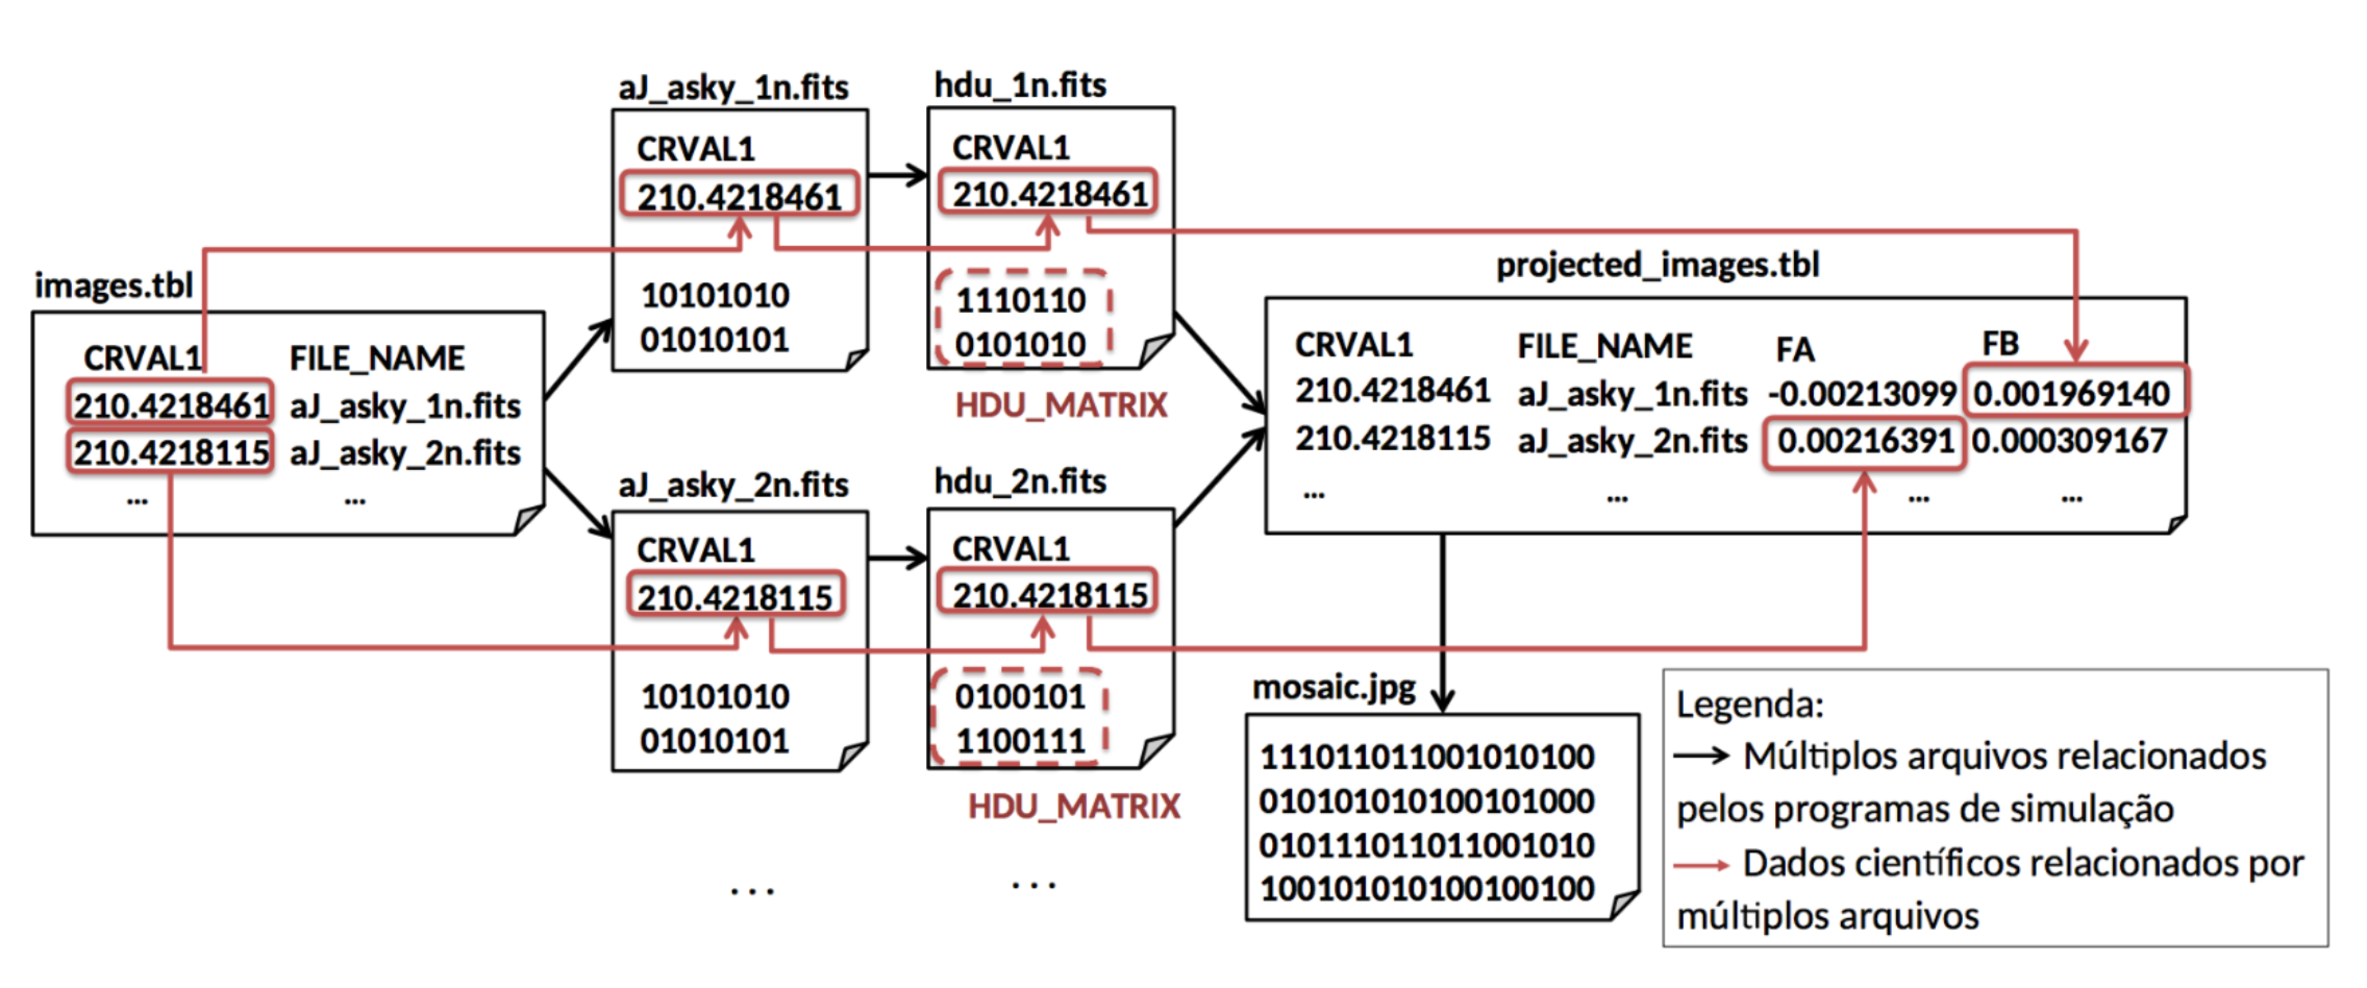
\includegraphics[width=\textwidth]{img/types-of-queries-1-2-3}
    \caption[Exemplo de análise de uma simulação de astronomia]{Exemplo de uma simulação de astronomia para análise de arquivos de dados científicos. Encontrada originalmente em~\cite{silva2015propostadoutorado}.}%
    \label{fig:types-of-queries-1-2-3}
\end{figure}

\section{Análise de dados científicos isolados}%
\label{sec:analise-de-dados-cientificos-isolados}

Consultas do \textbf{tipo 1} são caracterizadas pela \textbf{análise} (do inglês: \textit{parsing}) \textbf{de dados científicos}, encontrados em arquivos que foram produtos de uma simulação computacional, e envolve tipicamente a \textbf{extração} ou \textbf{interpretação} desses dados de acordo com o domínio da aplicação da simulação. É necessário conhecer a estruturação e~/~ou a codificação utilizada nesses arquivos para que seja possível acessá-los e extrair um significado semântico dos dados do mesmo; além disso, cada formato de arquivo possui programas específicos e peculiares para a sua análise e extração: por exemplo, um arquivo em formato de imagem tal como o \abbrev{PNG}{\textit{Portable Network Graphics}} PNG (Portable Network Graphics) pode ser analisado (visualizado) por um editor de imagens, enquanto que um arquivo em formato de música tal como o \abbrev{WAV}{Waveform Audio File Format} WAV (\textit{Waveform Audio File Format}) pode ser analisado (reproduzido) por um \textit{player} de áudio. Em particular, destaca-se que a semântica da análise --- reprodução, visualização, extração, etc --- é inerente ao tipo de arquivo analisado.

Esses dados e seus respectivos arquivos podem estar ou não em formato binário; por exemplo, um arquivo em formato \abbrev{JSON}{JavaScript Object Notation} JSON (JavaScript Object Notation) geralmente contém dados em formato de texto; enquanto que um arquivo FITS (Flexible Image Transport System)~\cite{greisen2002representations}, utilizado em astronomia, pode possuir parte de seus dados em formato binário assim como o NetCDF (Network Common Data Form)~\cite{rew1990netcdf}, utilizado em dinâmica de fluidos computacionais, e o HDF5~\cite{folk1999hdf5}, utilizado em várias aplicações distintas.

Consultas do tipo 1 são as mais simples de serem realizadas em relação às outras, pois elas são auto-contidas no que diz respeito aos dados científicos, isto é, apenas a presença desses dados é suficiente para que esse tipo de consulta possa ser realizado: não é necessária a especificação sobre o fluxo de dados da simulação computacional.

\perrotta{REVIEW: Extratores?? Como obtive os dados?}

\section{Rastreio de fluxos de arquivos}%
\label{sec:rastreio-de-fluxos-de-arquivos}

Consultas do \textbf{tipo 2} são caracterizadas pelo rastreio do \textbf{fluxo de arquivos}, que se relacionam através de transformações de dados. Elas são frequentemente apoiadas por sistemas de \textit{workflows} científicos, tais como o Chiron~\cite{ogasawara2011algebraic}, o Pegasus~\cite{deelman2005pegasus} e o Kepler~\cite{ludascher2006scientific}. Através desse tipo de consulta, que busca informações de proveniência retrospectiva, os usuários são capazes de rastrear, em uma míriade de arquivos de uma simulação computacional em larga escala, qual foi o fluxo de arquivos que gerou determinados conjuntos de dados finais a partir de quais conjutos de dados iniciais.

Um exemplo de ferramenta que é capaz de realizar consultas do tipo 2 é o \textit{NoWorkflow}~\cite{murta2014noworkflow} (do inglês: \textit{\textbf{n}ot \textbf{o}nly \textbf{workflow}}), que captura de forma transparente a proveniência de \textit{scripts} escritos na linguagem de programação Python. Essa captura é feita a nível de funções (subtorinas) da linguagem e, em particular, chamadas de sistema do tipo \emph{open} (=leitura de arquivos) presentes nos \textit{scripts} são capturadas, assim como os arquivos que lhe são passados como argumentos, que então são armazenados em um banco de dados relacional que identifica as relações (de entrada e de saída) entre esses arquivos. Dessa maneira, o \textit{NoWorkflow} possui toda a informação de proveniência retrospectiva~\cite{Pimentel2016} necessária para consultar o fluxo dos arquivos lidos e escritos durante a execução dos \textit{scripts}\footnote{Nesse contexto, um \textit{script} é análogo a um conjunto de transformações de dados, representando um programa científico.}.

Outra ferramenta que suporta consultas do tipo 2 é o \textit{YesWorkflow}~\cite{mcphillips2015yesworkflow}, que permite que os usuários façam anotações na forma de comentários especiais em seus \textit{scripts} e subsequentemente extrai e analisa esses comentários, representando os \textit{scripts} na forma de entidades e relações entre elas, formando e definindo um fluxo de dados. O \textit{YesWorkflow} pode ser utilizado em qualquer \textit{script}, não se limitando somente a Python, diferentemente do \textit{NoWorkflow}; mas, em contrapartida, ele requer anotações explícitas da parte do usuário, não sendo capaz de extrair informações de proveniência automaticamente como o \textit{NoWorkflow}~\cite{Pimentel2016}. Os comentários etiquetam regiões arbitrárias dos \textit{scripts}, associando valores a elas, os quais podem correlacionar e fazer associações a outras regiões; desse modo, um conjunto de comentários é capaz de especificar o fluxo de arquivos do fluxo de dados.

Citamos mais um exemplo de ferramenta que é capaz de realizar consultas do tipo 2, o Tigres~\cite{hendrix2016tigres}, que é inspirado no paradigma \textit{MapReduce} e suporta a criação de fluxos de dados sequenciais e paralelos. O Tigres é utilizado através de uma \abbrev{API}{Application Programming Interface} API (do inglês, Application Programming Interface) de \textit{templates} escrita em Python, com a qual o usuário define elementos do fluxo de dados e monitora a execução de programas científicos. Esses \textit{templates} funcionam como blocos de construção, que executam tarefas sequencialmente e geram informações de dependência e de proveniência entre os mesmos, tanto a nível prospectivo quanto a nível retrospectivo.

\section{Rastreio de fluxo de elementos de dados em múltiplos arquivos}%
\label{sec:rastreio-de-elemento-de-dados-em-multiplos-arquivos}

Consultas do \textbf{tipo 3} envolvem o rastreio de \textbf{elementos de dados relacionados} em \textbf{múltiplos arquivos}. Nesse sentido, são uma extensão das consultas do tipo 2, uma vez que é necessária uma granularidade mais fina para o fluxo, no nível de elementos de dados, e não apenas no nível do fluxo de arquivos.

O estado da arte no que diz respeito a soluções para análises de dados científicos em simulações científicas concentra-se hoje no apoio a consultas do tipo 1~\cite{alagiannis2012nodb,karpathiotakis2014adaptive,wu2009fastbit,folk1999hdf5,silva2015propostadoutorado} e do tipo 2~\cite{murta2014noworkflow,mcphillips2015yesworkflow,hendrix2016tigres,Pimentel2016}, como vimos em alguns exemplos nas seções anteriores. No entanto, algumas soluções para consultas do tipo 3 foram apresentadas nos últimos anos e vêm se consolidando recentemente.

Por exemplo, o \textit{NoWorkflow}, mencionado na \autoref{sec:rastreio-de-fluxos-de-arquivos}, também possui suporte a consultas do tipo 3, permitindo o rastreio de elementos de dados em nível de variáveis, de funções e de classes em \textit{scripts}, porém ele se limita somente a \textit{scripts} escritos na linguagem Python~\cite{murta2014noworkflow}

Outro paradigma que suporta consultas do tipo 3 é o da arquitetura ARMFUL, que é baseada em componentes e é instanciada, por exemplo, como o \textit{DfAnalyzer} em~\cite{silva2017raw}. Eles serão abordados detalhadamente no \autoref{chap:arquitetura-armful}.

\perrotta{REVIEW: DfAnalyzer (grupo) -- o que mais falar aqui?, CCPE (mais sistemas) - não entendi o que seria isso. Como expandir essa seção?}
  % !TEX encoding = UTF-8 Unicode
% -*- coding: UTF-8; -*-
% vim: set fenc=utf-8

\chapter{Arquitetura ARMFUL}%
\label{chap:arquitetura-armful}

Nesse capítulo é apresentada a arquitetura \abbrev{ARMFUL}{Analysis of Raw Data from Multiple Files} ARMFUL (do inglês: Analysis of Raw Data from Multiple Files; em tradução livre: Análise de Dados Científicos de Múltiplos Arquivos), introduzida recentemente em~\cite{silva2016situ,silva2017raw} pelo \abbrev{NACAD}{Núcleo Avançado de Computação de Alto Desempenho} Núcleo Avançado de Computação de Alto Desempenho (NACAD) da \abbrev{UFRJ}{Universidade Federal do Rio de Janeiro} UFRJ (Universidade Federal do Rio de Janeiro). Este capítulo também aborda o \textit{DfAnalyzer}, uma instância dessa arquitetura, implementada pelo mesmo laboratório.

\section{Visão geral}

A arquitetura \textbf{ARMFUL} tem suporte à extração de dados científicos, às técnicas de indexação e à análise de dados científicos a partir de múltiplos arquivos~\cite{silva2016situ} com o propósito de permitir o acesso direto a qualquer elemento ou região específica do espaço do fluxo de dados de uma simulação científica. Em outras palavras, ela permite a execução, \textit{off-line} e~/~ou \textit{on-line}\footnote{\textit{I.e.}, as consultas podem ser realizadas tanto \emph{após} as simulações científicas, quanto \emph{durante} as mesmas, respectivamente.}, de todos os três tipos de consultas apresentadas na \autoref{sec:tipos-de-consulta}. Essa flexibilidade e versatilidade na análise existe graças a uma \textbf{arquitetura de componentes}, que utiliza um banco de dados de proveniência para proporcionar um caminho de acesso entre o fluxo de dados e os dados científicos~\cite{silva2017raw}.

% Baseado na seção 5 de~\cite{silva2017raw}. Tentativa de tradução livre e de adaptação para o contexto desse trabalho.
A arquitetura ARMFUL funciona do seguinte modo: a gerência de conteúdos científicos é obtida a partir de dados científicos de arquivos, que então são correlacionados, em um repositório que é um SGBD relacional, através de dados de proveniência do seu respectivo fluxo de dados. Essa gerência de dados requer características que são específicas do domínio da simulação científica; por isso, modelos de dados de proveniência dessas simulações costumam ser representados em granularidade não-fina, \textit{i.e.}, as tabelas do SGBD possuem um grau de abstração relativamente alto para representar esses dados. Entretanto, consultas de proveniência possuem um valor analítico limitado caso não sejam relacionadas a elementos de dados específicos ao domínio da simulação computacional; contudo, esse relacionamento exige bastante esforço dos usuários de SGWfCs no que diz respeito a desenvolver, para cada domínio, um modelo de dados e programas científicos específicos para acessar, extrair e correlacionar os dados de domínio aos dados de proveniência. Nesse aspecto, a arquitetura ARMFUL contribui diminuindo o esforço necessário para capturar e representar esses dados de proveniência aravés da introdução e divisão de componentes genéricos e auto-contidos que modelam e correlacionam entre si, no mesmo banco de dados, (\(i\)) dados científicos específicos do domínio e (\(ii\)) proveniência.

Na \autoref{fig:armful-architecture-simplified}, podemos visualizar como é feita a representação e a divisão em componentes da arquitetura ARMFUL, que são os seguintes:

\begin{itemize}
    \item Banco de dados de proveniência;
    \item Extração de dados científicos;
    \item Indexação de dados científicos;
    \item Ingestão de dados de proveniência; e
    \item Processamento de consultas.
\end{itemize}

\begin{figure}[ht]
    \centering
    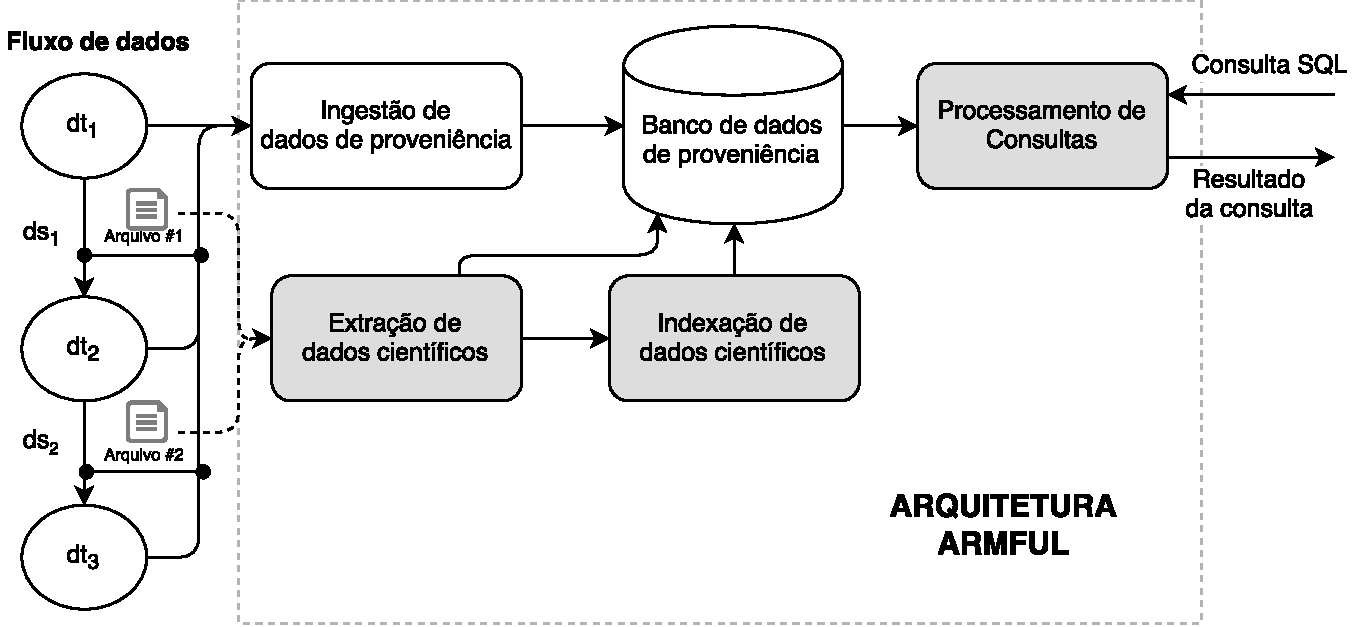
\includegraphics[width=\textwidth]{img/armful-architecture-simplified}
    \caption[Componentes da arquitetura ARMFUL]{Componentes da arquitetura ARMFUL. A cor branca representa as etapas relacionadas aos dados de proveniência, e a cor cinza tem relação com os dados científicos. Baseada em~\cite{silva2017raw}.}%
    \label{fig:armful-architecture-simplified}
\end{figure}

Os componentes na cor branca correspondem à captura e ao armazenamento de dados de proveniência em um banco de dados de proveniência. Em contrapartida, os componentes na cor cinza descrevem os passos responsáveis por: (\(i\)) extrair dados científicos de arquivos, (\(ii\)) gerar índices para os mesmos e (\(iii\)) permitir a consulta de proveniência \textbf{e} dados científicos a partir do mesmo banco de dados. Nas próximas subseções os componentes serão detalhados.

% Baseado na seção 5.1 de~\cite{silva2017raw}.
\subsection{Banco de dados de proveniência}%
\label{subsec:banco-de-dados-de-proveniencia}

O \textbf{banco de dados de proveniência}, que funciona como um repositório para os dados de proveniência, deve ser um \textbf{SGBD relacional}, e é responsável por armazenar, gerenciar e correlacionar (\(i\)) dados de proveniências e (\(ii\)) dados científicos, a fim de se beneficiar do suporte analítico de consultas do fluxo de dados. Além disso, SGBDs possuem solidez, confiabilidade e segurança, oriundas de uma experiência de mais de 30 anos de estudos científicos e aplicações no mundo real, provendo estratégias e algoritmos bem conhecidos que garantem atomicidade, consistência, isolamento e durabilidade (ACID) em transações, além de possuir soluções consolidadas e robustas no que diz respeito a recuperação de dados e controle concorrente de acesso~\cite{ozsu2011principles}.

\subsection{Extração e indexação de dados científicos}%
\label{subsec:extracao-e-indexacao-de-dados-cientificos}

O \textbf{componente de extração de dados científicos} tem o objetivo de ler o conteúdo de arquivos científicos, analisá-lo e então recuperar parte do conteúdo selecionado que é relevante de acordo com os atributos especificados pelo usuário. Para que esse objetivo seja completado, quatro etapas devem ser seguidas:

\begin{itemize}
    \item \textbf{leitura do conteúdo}: acesso aos arquivos científicos e leitura do seu conteúdo;
    \item \textbf{tokenização}: investigação de metadados relacionados à especificação do formato de arquivo, visando verificar se os dados científicos obtidos na etapa anterior correspondem ao domínio da simulação computacional processada atualmente;
    \item \textbf{filtragem de conteúdo}: a especificação do usuário é responsável por definir e restringir o que deve ser analisado e armazenado no banco de dados de proveniência, isto é, essa etapa evita armazenar atributos desnecessários, que não serão utilizados na próxima etapa;
    \item \textbf{análise}: conversão de cada dado científico filtrado em uma estrutura de dados apropriada para ser armazenada no SGBD.
\end{itemize}

O \textbf{componente de indexação de dados científicos} é opcional e visa indexar um conteúdo específico dos arquivos científicos a fim de agilizar o tempo de acesso direto a determinadas regiões do espaço de dados científicos através da gerência de metadados correlacionados ao fluxo de dados. A criação de índices é realizada segundo um algoritmo de indexação previamente definido, \textit{e.g.} indexação por \textit{bitmap} ou indexação posicional.

O volume de dados científicos que é gerado durante a execução de uma simulação computacional é um fator determinante para a definição da melhor estratégia para a representação desses dados~\cite{silva2015propostadoutorado}: em simulações que geram um pequeno volume de dados em cada transformação de dados e que possuem poucos atributos, a extração e ingestão (\textit{i.e.}, carga no banco de dados de proveniência) de dados científicos \emph{diretamente} com seus próprios valores de dados costuma ser uma abordagem melhor. Em contrapartida, em um cenário no qual um grande volume de dados --- com estruturas de dados complexas --- precisa ser capturado, o componente de indexação é fortemente recomendado.

\subsection{Ingestão de dados}%
\label{subsec:ingestao-de-dados}

O \textbf{componente de ingestão de dados} é responsável por coletar a \textbf{proveniência} do fluxo de dados, selecionando, manipulando e armazenando (\textit{i.e.} realizando a carga dos valores assumidos pelos atributos) convenientemente as informações referentes aos arquivos e dados científicos no banco de dados mencionado na \autoref{subsec:banco-de-dados-de-proveniencia}~\cite{silva2015propostadoutorado}. Em outras palavras, esse componente é responsável por alimentar e popular o SGBD com informações de dados de proveniência que serão posteriormente utilizadas para auxiliar o componente de processamento de consultas, que será discutido na próxima seção. Esse componente interfaceia diretamente com todo item do fluxo de dados.

A captura de dados de proveniência deve ser realizada com uma granularidade fina, de modo a apoiar e capturar os dois tipos de análises exploratórias em arquivos de dados científicos mencionadas na \autoref{subsec:categorias-de-dados-de-proveniencia} (proveniência prospectiva e retrospectiva). Além disso, também deve realizar a gerência do fluxo de dados nos níveis físico e lógico.

\subsection{Processamento de consultas}

Uma vez que todos os dados científicos e toda a proveniência sejam devidamente capturadas e armazenadas em um repositório SGBD, os usuários poderão consultá-los para apoiar (refutar ou validar) suas hipóteses científicas~\cite{silva2015propostadoutorado}. Nesse contexto, o \textbf{componente de processamento de consultas} é responsável por prover um mecanismo de consultas à proveniência e aos dados científicos armazenados em um banco de dados de proveniência compatível com um modelo de dados adequado. O comportamento desse componente é variável, dependendo da estratégia utilizada nos componentes anteriores --- de extração e de indexação. Uma vez que esse componente utiliza um SGBD para o armazenamento dos dados de proveniência, somente tipos de consultas que são permitidas e disponíveis pelo SGBD podem ser realizadas. Em particular, e como consequência disso, as consultas são comumente especificadas em uma linguagem de alto nível, como a linguagem declarativa SQL.

O processador de consultas é um componente bastante importante, já que é a principal interface entre os usuários e uma instância da arquitetura ARMFUL, e todas as consultas ao banco de dados são iniciadas (e especificadas) a partir dele.

\section{DfAnalyzer: uma instância da arquitetura ARMFUL}%
\label{sec:dfanalyzer-uma-instancia-da-arquitetura-armful}

\subsection{Visão Geral}%
\label{subsec:dfanalyzer-visao-geral}

Como vimos na seção anterior, a arquitetura ARMFUL é uma \textbf{abstração} que define e especifica componentes a fim de prover um mecanismo capaz de realizar consultas a um banco de dados, cujos dados de proveniência, execução e domínio foram oriundos de uma simulação computacional. Dito isso, o \textbf{DfAnalyzer} é uma \textbf{instância da arquitetura ARMFUL}; em outras palavras, ele consiste em uma implementação dessa arquitetura. Ele foi originalmente introduzido em~\cite{silva2016situ}. Os principais componentes do DfAnalyzer são abordados nas próximas subseções.

\perrotta{TODO: Descrição geral / overview do DfAnalyzer, in order to replace the former sedimentation solver simulation text}

\subsection{Provenance Data Gatherer (PDG)}

O \textbf{Provenance Data Gatherer} (PDG) é o componente do DfAnalyzer responsável por \textbf{capturar dados de proveniência} (\textit{c.f.} \autoref{subsec:ingestao-de-dados}) assim como dados específicos do domínio a partir do código fonte da aplicação, gerando um arquivo JSON com o conteúdo extraído e as suas respectivas dependências de dados~\cite{silva2016situ}. Após a captura, a proveniência e os dados de domínio são carregados em um banco de dados que é compatível com um esquema (do inglês \textit{schema}) pré-definido e que é gerenciado pelo SGBD MonetDB~\cite{boncz2008breaking}, que consiste em um banco de dados orientado a colunas compatível com a linguagem SQL.

O motivo do MonetDB ter sido escolhido como o SGBD para a gerência e o armazenamento dos dados de proveniência deve-se principalmente ao fato do mesmo ser orientado e otimizado para a consulta de dados através de colunas --- diferentemente da maioria dos SGBDs tradicionais, como o MySQL e o SQLite, que são orientados a linhas. Isso é importante pois, em geral, o principal interesse nas consultas das simulações computacionais consiste na obtenção de apenas um subconjunto dos atributos presentes.
% https://www.monetdb.org/Documentation/Manuals/SQLreference/Indices
Além disso, o MonetDB trata suas cláusulas de indexação de forma peculiar e dinâmica: diferentemente de SGBDs tradicionais, essas cláusulas são postergadas, interpretadas meramente como \textit{hints}, sendo o MonetDB o responsável por tomar as decisões finais de manutenção e de criação de índices, visando assim acelerar o posterior acesso aos dados~\cite{url:monetdb}.

Existem duas fontes de proveniência para o PDG. Uma é a \textit{libMesh-sedimentation solver}, mencionada anteriormente na \autoref{subsec:dfanalyzer-visao-geral}, que contribui com dados de domínio obtidos diretamente do código fonte do resolvedor de dinâmica de fluidos computacionais. A outra é o ParaView Catalyst~\cite{ayachit2015paraview}, que é uma biblioteca com o qual o DfAnalyzer pode comunicar-se para aproveitar-se dos dados gerenciados em memória por ele e relacioná-los com o banco de dados de proveniência, além de prover recursos de visualização e de processamento de dados. O Paraview Catalyst pode ser utilizado para extrair dados que estão em memória, complementando a \textit{libMesh-sedimentation} e gerar visualizações de regiões de interesse.

\subsection{Raw Data Extractor (RDE)}

Uma vez que o PDG especializa-se em coletar proveniência e dados de domínio, o \textbf{Raw Data Extractor} (RDE) o complementa, sendo o componente responsável por \textbf{extrair} os dados científicos que estão presentes em arquivos científicos (\textit{c.f.} \autoref{subsec:extracao-e-indexacao-de-dados-cientificos}). Esses arquivos usualmente mantêm seus dados em formato binário, total ou parcialmente, sendo responsabilidade do RDE a leitura, filtragem e análise do conteúdo desses dados, transformando-os em um formato adequado para ser armazenado nos tipos e tabelas disponíveis no MonetDB. Dependendo da aplicação e da simulação científica, o conteúdo desses arquivos científicos pode ser ora armazenado diretamente no SGBD, ora armazenado indiretamente, através de ponteiros (referências de arquivos), ou estruturas de dados em formatos intermediários de representação.

\subsection{Raw Data Indexer (RDI)}

O \textbf{Raw Data Indexer} (RDI) é o componente do DfAnalyzer responsável por indexar dados científicos presentes em arquivos, com o objetivo de permitir o acesso eficiente aos dados durante a execução das consultas pelos usuários, diminuindo o tempo médio delas (\textit{c.f.} \autoref{subsec:extracao-e-indexacao-de-dados-cientificos}). O RDI é comumente utilizado para indexar estruturas de dados mais complexas, como matrizes e malhas esparsas, que demandam um custo de tempo para a carga de dados em uma base de dados muito grande. Outro fator para o uso de técnicas de indexação consiste na dificuldade de representar determinadas estruturadas de dados em um SGBD, por exemplo. Entretanto, esse trabalho não contempla o uso do RDI nos experimentos realizados, nem requer uma descrição detalhada desse componente, pois a implementação de indexação de dados científicos não foi considerada para o desenvolvimento do processador de consultas deste projeto de graduação.

\subsection{Query Processor (QP)}

O \textbf{Query Processor} (QP) é o componente responsável por auxiliar os usuários a \textbf{submeterem consultas} na linguagem SQL ao banco de dados de proveniência~\cite{silva2016situ}, realizar a validação dessas consultas --- por exemplo, se a sintaxe e~/~ou se os nomes dos atributos de dados estão corretos --- e então finalmente retornar e exibir os resultados das mesmas. Com o objetivo de facilitar a execução de consultas por novos usuários, sem a necessidade de que eles tenham que aprender todos os aspectos da sintaxe da linguagem SQL, uma nova forma simplificada de especificação e de descrição de consultas foi desenvolvida, a qual traduz e converte a consulta do usuário para SQL, e é essa conversão que é enviada ao MonetDB, o qual retorna os resultados para o usuário.

Essa conversão possui duas vantagens básicas: a primeira, mencionada anteriormente, é a facilidade para novos usuários interagirem com o DfAnalyzer, de forma mais intuitiva e direta, sem a necessidade de descrever uma consulta em SQL completa e válida, e nem a necessidade de conhecer completamente todos os dados do domínio. A segunda é a possibilidade do QP realizar otimizações na consulta antes de enviá-la diretamente ao MonetDB. Por exemplo, em dada consulta, a cláusula \textsc{FROM} pode ser otimizada, filtrando tabelas que não sejam realmente necessárias na consulta em questão, diminuindo a sobrecarga ao SGBD e recuperando apenas os dados realmente necessários para o sucesso da consulta.

O QP é capaz de realizar todos os três tipos de consultas mencionados anteriormente na \autoref{sec:tipos-de-consulta}: \((i)\) análise de dados científicos isolados de um único arquivo; \((ii)\) rastreamento de fluxos de múltiplos arquivos relacionados; e \((iii)\) rastreamento de elementos de dados relacionados e múltiplos arquivos. 
A principal contribuição deste trabalho encontra-se especificamente na implementação deste componente, a qual será detalhadamente discutida no \autoref{chap:rastros-de-proveniencia}.
  % !TEX encoding = UTF-8 Unicode
% -*- coding: UTF-8; -*-
% vim: set fenc=utf-8

\chapter{Abordagem para análise de rastros de proveniência}%
\label{chap:rastros-de-proveniencia}

% ilustrar com query SQL, tabela, grafo (img)

\section{Visão geral sobre a análise de rastros de proveniência}

 % definição, etc
 
\section{Tipos de rastros de proveniência}

% explicação + exemplo + complemento de uma (sub)seção anterior

\subsection{Físico}

\subsection{Lógico}

\subsection{Híbrido}

% \section{DfAnalyzer: Uma instanciação da arquitetura ARMFUL para análise dos rastros de proveniência}

\section{Query Processor}

O Query Processor foi implementado na linguagem de programação Java...

\perrotta{TODO: EXPAND}

\perrotta{TODO: Mencionar o pré-processamento e as otimizações que fiz}

\section{Algoritmos utilizados}

\subsection{Detecção das últimas transformações de dados}

O \autoref{lst:algorithm-last-transformations} demonstra como obter as \textbf{últimas transformações de dados} \texttt{transformations} de um fluxo de dados \( D \), isto é, as transformações de dados \(dt\) as quais não possuem nenhuma outra transformação de saída após as mesmas. A ideia do algoritmo é bastante simples: basta checar todas as dependências de dados \( \phi \) --- do conjunto de dependência de dados do fluxo de dados \( D.\Phi \) --- cujo \( dt_{\textrm{next}} \) é nulo, e tomar o \( dt_{\textrm{previous}} \) das mesmas.

% https://tex.stackexchange.com/questions/73231/avoid-page-breaks-in-lstlistings
\begin{minipage}[c]{0.95\textwidth}
\begin{lstlisting}[language=pseudocode,label={lst:algorithm-last-transformations},caption={[Detecção das últimas transformações de dados]Detecção das útimas transformações de dados em uma especificação de fluxo de dados.}]
function getLastTransformations(%\(D\)%):
    transformations %\leftarrow% {}
    for each %\phi% %\in% %\(D.\Phi\)% do:
        if %$\phi.dt_{\texttt{next}} == \varnothing$% then:
            transformations %\leftarrow% transformations + 
        end if
    end do
    return transformations
end function
\end{lstlisting}
\end{minipage}

A complexidade de tempo do algoritmo é linear da ordem de \( O(\#(\Phi)) \), isto é, proporcional ao número de dependência de dados do fluxo de dados \( D \), e as transformações retornadas pelo algoritmo são armazenadas em uma simples lista encadeada, já que não é necessário ter acesso aleatório a essa estrutura de dados. Entretanto, na prática, esse algoritmo é aplicado \textit{on-the-fly}, no momento em que o fluxo de dados é construído e instanciado no QP.

\subsection{Detecção das trilhas de transformações}%
\label{subsec:deteccao-das-trilhas-de-transformacoes}

O \autoref{lst:algorithm-transformation-tracks} demonstra como obter as \textbf{trilhas de transformações} \texttt{dtTracks} de um fluxo de dados \( D \). As trilhas são uma maneira natural de separar e agrupar transformações de dados em vários subconjuntos, definidos e limitados através de separações (\textit{splits}) em \( D \). Tais separações existem no grafo do fluxo de dados em interseções de transformações que possuem mais de uma transformação de entrada ou de saída (\textit{i.e.}, grau do vértice maior do que 1). Por exemplo, na \autoref{fig:transformation-tracks}, podemos visualizar um exemplo de divisão e agrupamento de transformações de dados em trilhas.

\begin{figure}[htb]
    \centering
    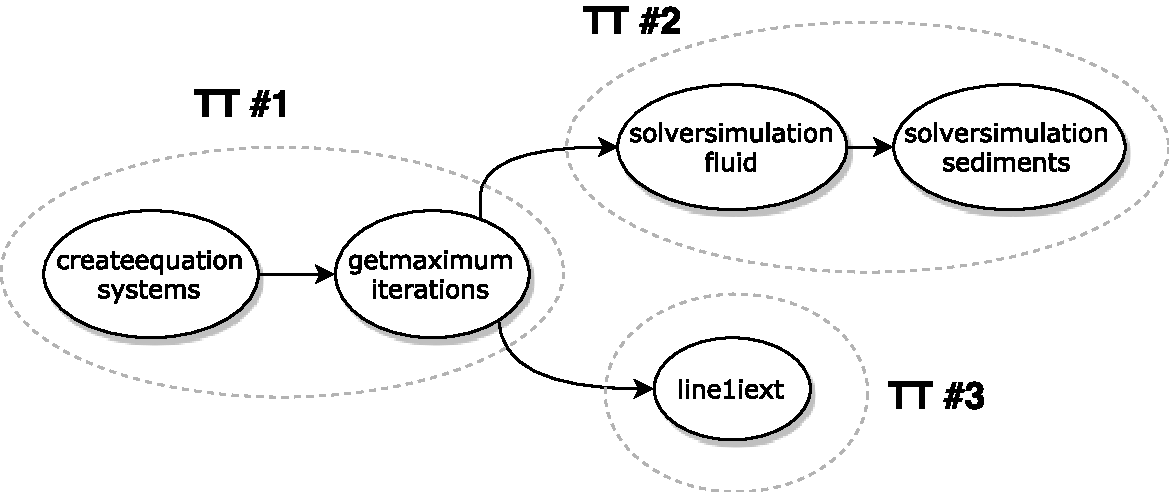
\includegraphics[width=\textwidth]{img/transformation-tracks}
    \caption[Exemplo de detecção das trilhas de transformações.]{Exemplo de detecção das trilhas de transformações de um fluxo de dados. Na figura existem três trilhas de transformações (\textsc{TT}).}%
    \label{fig:transformation-tracks}
\end{figure}

O algoritmo começa com as últimas transformações de \( D \) (encontradas no \autoref{lst:algorithm-last-transformations}), e caminha em direção às primeiras transformações de \( D \). A ideia principal é realizar a detecção do fim --- e, portanto, do início --- de cada trilha de transformação, que pode acontecer em várias situações: \textit{e.g.}, sempre que o grau de saída do vértide de transformação for maior do que 1, indicando que a transformação em questão possui várias transformações de saída.

\begin{minipage}[c]{0.95\textwidth}
\begin{lstlisting}[language=pseudocode,label={lst:algorithm-transformation-tracks},caption={[Detecção das trilhas de transformações]Detecção do rastro do fluxo de dados no nível de trilhas de transformações.}]
function getTransformationTracks(%\(D\)%):
    dtTracks %\leftarrow% {}
    lastDts %\leftarrow% getLastTransformations(%\(D\)%) %\quad%# %\autoref{lst:algorithm-last-transformations}%
    queue %\leftarrow% {}
    queue.push(lastDts)
    while queue is not empty do:
        dt %\leftarrow% queue.pop()
        nextDts %\leftarrow% getNextTransformations(%\(D\)%, dt)
        if lastDts.contains(dt)
           or hasManyOutputDatasets(%\(D\)%, dt)
           or hasManyNextTransformations(%\( D \)%, dt)
           or anyTransformationHasManyInputDatasets(%\(D\)%, nextDts)
           then:
            track %\leftarrow% new TransformationTrack()
            track.addTransformation(dt)
            dtTracks %\leftarrow% dtTracks + {track}
        else then:
            track %\leftarrow% getTransformationTrack(dtTracks, nextDts)
            track.addTransformation(dt)
        end if
        previousDts %\leftarrow% getPreviousTransformations(%\(D\)%, dt)
        queue.push(previousDts)
    end do
    return dtTracks
end function
\end{lstlisting}
\end{minipage}

A complexidade de tempo do algoritmo é linear da ordem de \( O(\#(T)) \), isto é, proporcional ao número de transformações de dados presentes em \( D \). As trilhas de transformações são armazenadas em listas encadeadas de transformações.

\subsection{Detecção das trilhas de conjuntos de dados}

O \autoref{lst:algorithm-dataset-tracks} tem como função obter as \textbf{trilhas de conjuntos de dados} \texttt{dsTracks} de um fluxo de dados \( D \). O conceito de trilha de conjuntos de dados é análogo ao de trilha de transformações de dados, mencionado na \autoref{subsec:deteccao-das-trilhas-de-transformacoes}: é uma forma de dividir e agrupar conjuntos de dados em diversos subconjuntos.

O algoritmo funciona com base no \autoref{lst:algorithm-transformation-tracks}: uma vez tomadas as trilhas de transformações de dados, é trivial obter cada uma das trilhas de conjuntos de dados a partir de cada uma delas. Para isso, basta tomar a união de todos os conjuntos de dados adjacentes (\textit{i.e.} anteriores e posteriores) a todas as transformações de dados de uma trilha de transformações.

\begin{minipage}[c]{0.95\textwidth}
\begin{lstlisting}[language=pseudocode,label={lst:algorithm-dataset-tracks},caption={[Detecção das trilhas de conjuntos de dados]Detecção do rastro do fluxo de dados no nível de trilhas de conjuntos de dados.}]
function getDatasetTracks(%\(D\)%):
    dsTracks %\leftarrow% {}
    dtTracks %\leftarrow% getTransformationTracks(D) %\quad%# %\autoref{lst:algorithm-transformation-tracks}%
    for each dtTrack %\in% dtTracks do:
        dsTrack %\leftarrow% {}
        for each dt %\in% dtTrack do:
            if dsTrack is empty then:
                nextDss %\leftarrow% getNextDatasets(%\(D\)%, dt)
                dsTrack %\leftarrow% dsTrack + {nextDss}
            end if
            previousDss %\leftarrow% getPreviousDatasets(%\(D\)%, dt)
            dsTrack %\leftarrow% dsTrack + {previousDss}
        end do
        dsTracks %\leftarrow% dsTracks + {dsTrack}
    end do
    return dsTracks
end function
\end{lstlisting}
\end{minipage}

A complexidade de tempo do algoritmo é a mesma do algoritmo do \autoref{lst:algorithm-transformation-tracks}: linear da ordem de \( O(\#(T)) \), e as trilhas de conjuntos de dados são também armazenadas em listas encadeadas de conjuntos de dados.

\subsection{Obtenção de múltiplos mapeamentos de atributos entre dois conjuntos de dados}

O \autoref{lst:algorithm-attribute-mappings} demonstra como obter \textbf{múltiplos mapeamentos de atributos}...

\perrotta{TODO: introduction with caption repeating + algorithm explanation. Reiterate the definition of mapeamentos de atributos (seção 2, das definições).}

\begin{minipage}[c]{0.95\textwidth}
\begin{lstlisting}[language=pseudocode,label={lst:algorithm-attribute-mappings},caption={[Obtenção de múltiplos mapeamentos de atributos]Obtenção de múltiplos mapeamentos de atributos entre dois conjuntos de dados adjacentes.}]
function getAttributesMapping(dt,%\(\textrm{ds}_{\textrm{input}}\)%,%\(\textrm{ds}_{\textrm{output}}\)%,type)
   attrs %\leftarrow% {}
   if type == physical then:
       attrs %\leftarrow% attrs + {t.getInstanceAttribute()}
   else:
       for each inAttr %\in% %\(\textrm{ds}_{\textrm{input}}\).A% do:
           for each outAttr %\in% %\(\textrm{ds}_{\textrm{output}}\).A% do:
               if inAttr.name == outAttr.name
                  and inAttr.type == outAttr.type then:
                   attrs %\leftarrow% attrs + {inAttr}
               end if
           end for
       end do
   end if
   %\mu% %\leftarrow% attributesMapping(attrs,dt,%\(\textrm{ds}_{\textrm{input}}\)%,%\(\textrm{ds}_{\textrm{output}}\)%)
   return %\mu%
end function
\end{lstlisting}
\end{minipage}

\perrotta{TODO: complexity and data structures}

\subsection{depthFirstSearch from PathFinder.java}

\perrotta{TODO: everything. Autoref code label, Bold title, Introduction with caption repeating + algorithm explanation. Later: Complexity, data structures.}

\subsection{findPaths from PathFinder.java}

\perrotta{TODO: everything}

\subsection{generateSqlQuery from QueryCreator.java}

\perrotta{TODO: everything}

\section{Um exemplo}

\perrotta{como rodar o algoritmo -- explicar a assinatura da função principal e exemplos de uso (chamadas)}
  % !TEX encoding = UTF-8 Unicode
% -*- coding: UTF-8; -*-
% vim: set fenc=utf-8

\chapter{Experimentos}%
\label{chap:experimentos}

Esse capítulo apresenta alguns exemplos de experimentos e de simulações computacionais com base em uma aplicação do DfAnalyzer no campo de sedimentação de dinâmica de fluidos computacionais~\cite{silva2016situ}, os quais foram executados a fim de ilustrar a implementação e a utilização do Query Processor --- apresentado no \autoref{chap:rastros-de-proveniencia} ---, assim como os resultados obtidos com as consultas realizadas nos mesmos.

\section{Simulação computacional em sedimentação}

O DfAnalyzer (\textit{c.f.} \autoref{sec:dfanalyzer-uma-instancia-da-arquitetura-armful}) utiliza a \textit{libMesh}, uma biblioteca \textit{open-source} implementada na linguagem C++, desenvolvida para facilitar a simulação de aplicações paralelas de refinamento de malhas e elementos finitos adaptativos~\cite{boncz2008breaking}, em um resolvedor chamado \textit{libMesh-sedimentation}. O propósito dessa aplicação é simular a turbidez e perturbação de correntes de fluidos tipicamente encontradas em processos geológicos. Os sedimentos que são transportados devido à dinâmica e ao movimento dos fluidos computacionais são descritos por um modelo matemático que resulta da equação de incompressibilidade de Navier-Stokes (fluido) combinada com uma equação de transporte dominada por advecção (concentração de sedimentos). A \textit{libMesh-sedimentation} emprega um método de elementos finitos de multi-escala variacional no qual uma abordagem escalonada é utilizada para representar e simular a evolução do tempo nas equações de acoplamento entre o fluido e os sedimentos. 

Nessa aplicação os usuários empregam simulações complexas nas quais grandezas de interesse, tais como resíduos e estimativas de erros, são utilizadas para controlar de forma fina o êxito e a performance da execução~\cite{silva2016situ}. Por exemplo, a convergência ou divergência de valores de determinadas grandezas e atributos, ao longo do tempo, é uma potencial e rica fonte de informação sobre o andamento da simulação computacional. Contudo, em geral, não basta analisar uma única grandeza: frequentemente faz-se necessária a análise dos dados científicos de múltiplos arquivos, gerados em diferentes passos durante a execução do \textit{solver}. Nesse cenário a análise é possibilitada pelo DfAnalyzer o qual, devido a sua arquitetura em componentes herdada da ARMFUL, permite que consultas relacionadas a proveniência e aos dados científicos de múltiplos arquivos e transformações de dados sejam realizadas \textit{on-line}, ainda durante a execução da simulação computacional.

Neste capítulo realizamos várias consultas com um fluxo de dados \(D^{\dagger}\) baseado no \textit{solver} de \textbf{simulação de sedimentação de dinâmica de fluidos computacionais} mencionado nos parágrafos anteriores. Esse fluxo de dados \(D^{\dagger}\) está ilustrado na \autoref{fig:experiments-dataflow}.

\begin{figure}[!htb]
    \centering
    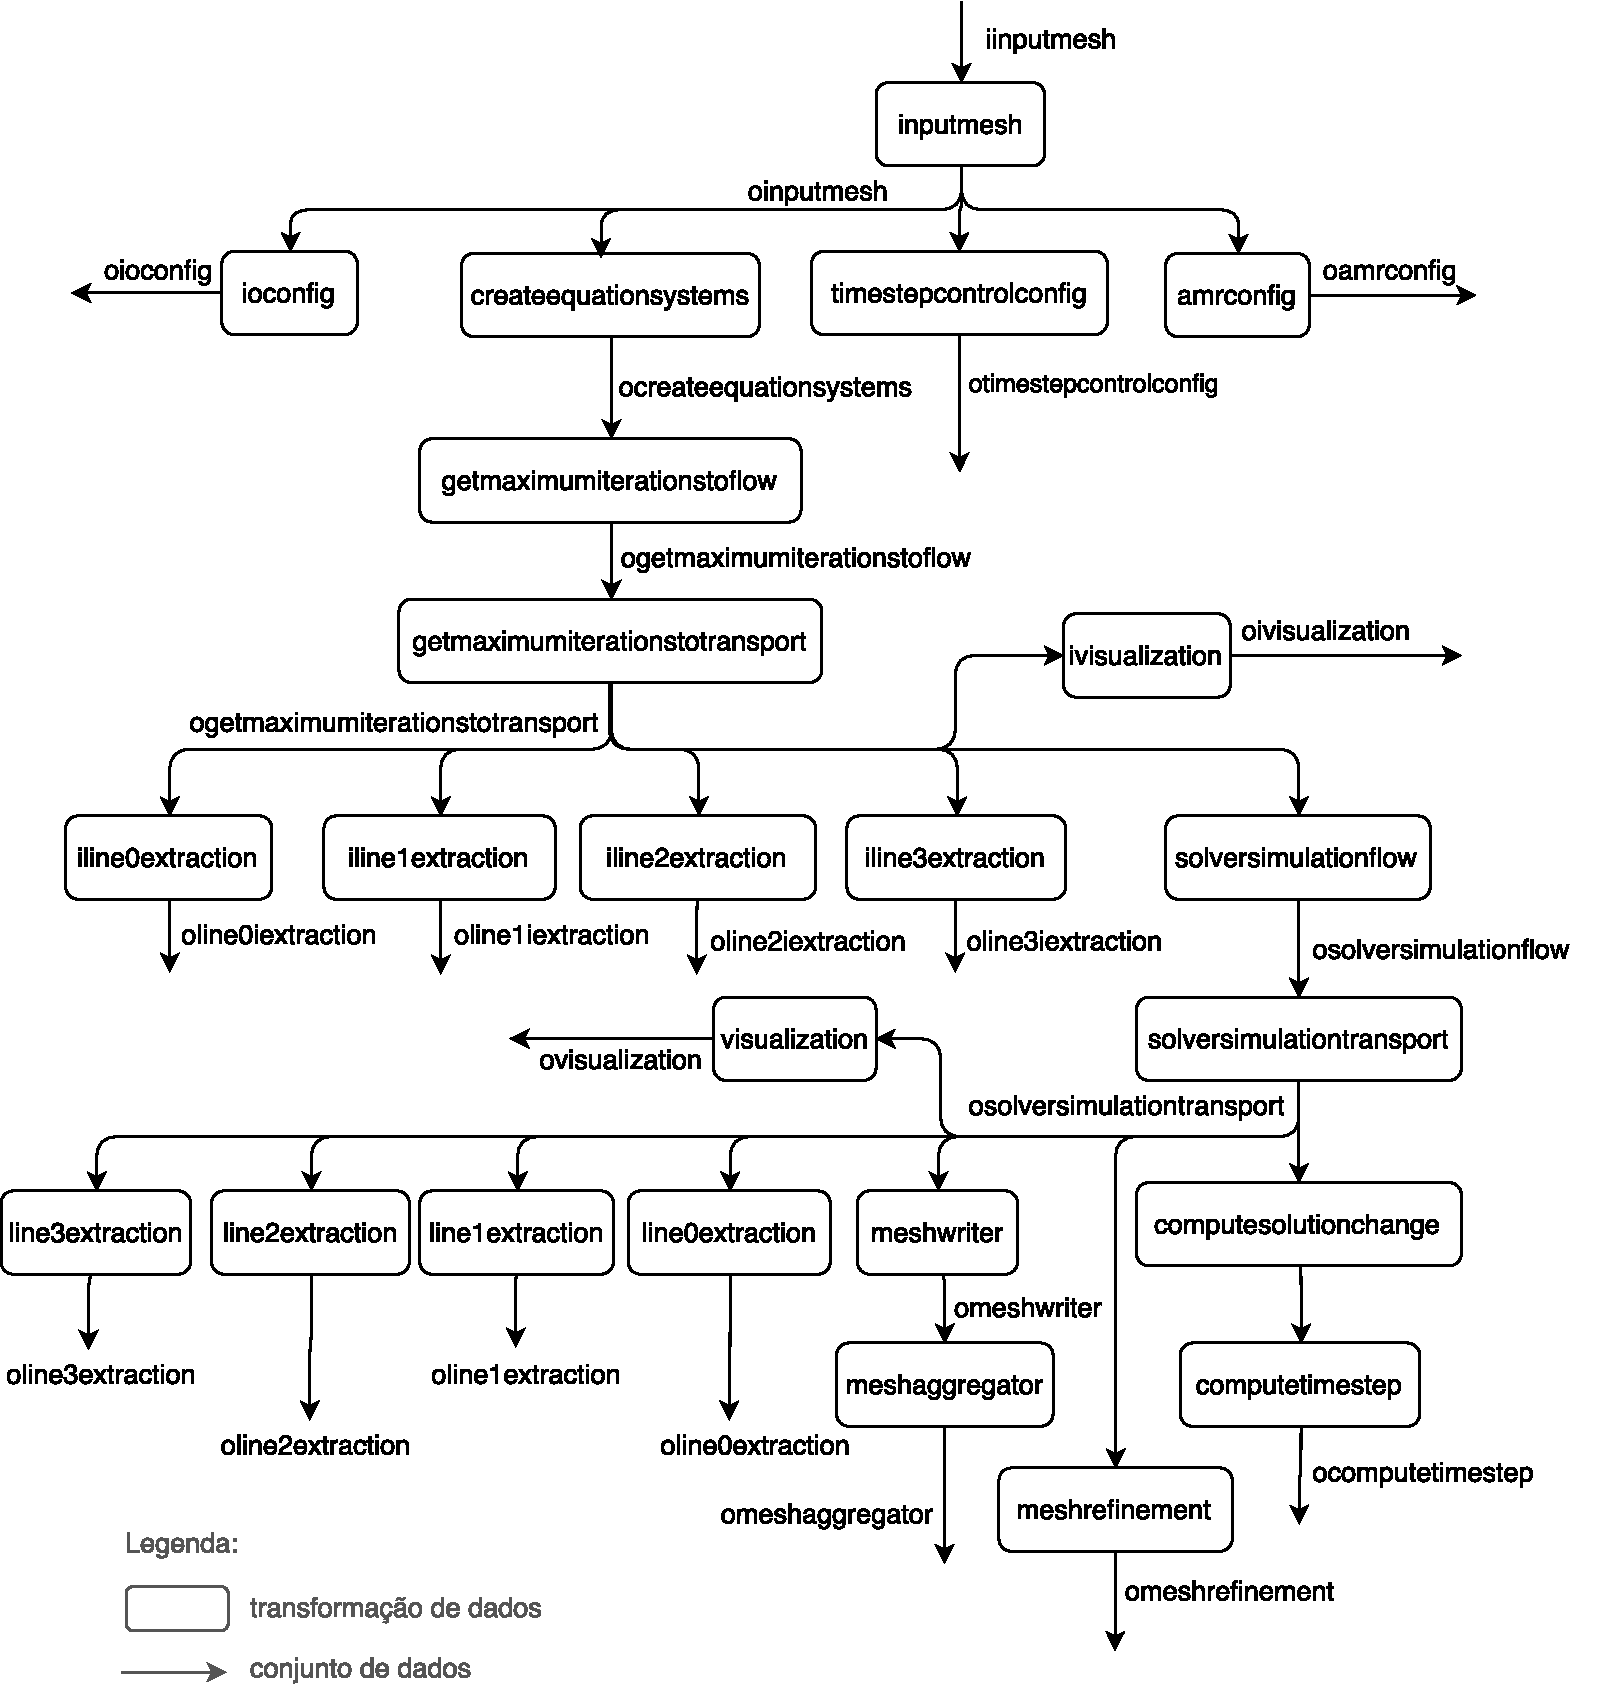
\includegraphics[width=\textwidth]{img/experiments-dataflow}
    \caption[Fluxo de dados $D^{\dagger}$ utilizado nos experimentos]{Fluxo de dados $D^{\dagger}$ utilizado nos experimentos e nas consultas do \autoref{chap:experimentos}.}%
    \label{fig:experiments-dataflow}
\end{figure}

Devido à grande quantidade de conjuntos de dados \(S^{\dagger}\) de \(D^{\dagger}\), não listamos todos os atributos de dados de \(S^{\dagger}\). No entanto, para fins de ilustração, alguns atributos de dados de \(S^{\dagger}\) podem ser visualizados na \autoref{tab:experiments-data-attributes}.

\begin{table}[htb]
    \centering
    \begin{tabular}{c|c|c|c}
\textbf{Conjunto de dados}                  & \textbf{Atributo de dados} & \textbf{Tipo}   & \makecell{\textbf{Exemplo} \\ \textbf{de Valor}}             \\ \hline
\multirow{3}{*}{osolversimulationtransport} & time                       & \makecell{ponto \\ flutuante} & 1e-05                                  \\ \cline{2-4}
                                            & t\_step                    & inteiro         & 0                                      \\ \cline{2-4}
                                            & meshwriter\_task\_id       & inteiro         & 17                                     \\ \hline
\multirow{2}{*}{omeshaggregator}            & xdmf                       & arquivo         & \texttt{\textasciitilde/output\_48.xmf}             \\ \cline{2-4}
                                            & n\_processors              & inteiro         & 480                                    \\ \hline
omeshrefinement                             & first\_step\_refinement    & booleano        & falso                                  \\ \hline
ovisualization                              & png                        & arquivo         & \texttt{\textasciitilde/image\_99.png} \\ \hline
oinputmesh                                  & mesh\_file                 & arquivo         & \texttt{\textasciitilde/necker3d.mesh}               \\ \hline
otimestepcontrolconfig                      & model\_name                & string          & PC11                                  
    \end{tabular}
    \caption[Exemplos de alguns atributos de dados de \(S^{\dagger}\)]{Exemplos de alguns atributos de dados de \(S^{\dagger}\).}%
    \label{tab:experiments-data-attributes}
\end{table}

% \silva{REVIEW: que tipos de arquivos ou dados são coletados na libMesh-sedimentation?. No solver, capturamos dados referentes ao resíduo do solver ao resolver as equações para o fluido e os sedimentos. Para a gerência de arquivos, consideramos os raw data files nos formatos XDMF e HDF5.}

\perrotta{TODO: citar artigo do email}

\section{Experimentos}

As consultas dos experimentos das próximas subseções, relacionadas ao Query Processor, foram executadas em um computador com as seguintes especificações:

\begin{itemize}
	\item Macbook Pro Retina 2015, com o sistema operacional macOS Sierra 10.12.6;
    \item Processador Intel Core i5 2,7~GHz, com 4~CPUs;
    \item 8~GB de memória RAM do tipo DDR3.
\end{itemize}

Quatro consultas foram realizadas, cada uma das quais com diversos parâmetros para a função \texttt{generateSqlQuery} (\textit{c.f.} \autoref{subsec:geracao-da-consulta-em-sql}).

\subsection{Consulta \#1}

% Tempo: rodar 4 vezes, tirar a média das 3 últimas

\perrotta{TODO: observação: GROUP BY}

\begin{table}[htb]
    \centering
    \begin{tabular}{c|c}
\textbf{Argumento}          & \textbf{Valor} \\ \hline
\texttt{D}                  & $D^{\dagger}$ \\
\texttt{dsOrigins}          & \{\texttt{osolversimulationtransport}\} \\
\texttt{dsDestinations}     & \{\texttt{oline2extraction}, \texttt{omeshwriter}\} \\
\texttt{type}               & physical \\
\texttt{projections}        & \{\texttt{osolversimulationtransport.time}, \texttt{AVG(oline2extraction.d)}\} \\
% \texttt{selections}         & \varnothing \\
\texttt{dsIncludes}         & \varnothing \\
\texttt{dsExcludes}         & \varnothing \\
    \end{tabular}
    \caption[Argumentos da função \texttt{generateSqlQuery} para a consulta \#1]{Especificação dos argumentos da função \texttt{generateSqlQuery} para a consulta~\#1.}%
    \label{tab:experiments-1-especificacao}
\end{table}

\begin{figure}[htb]
    \centering
    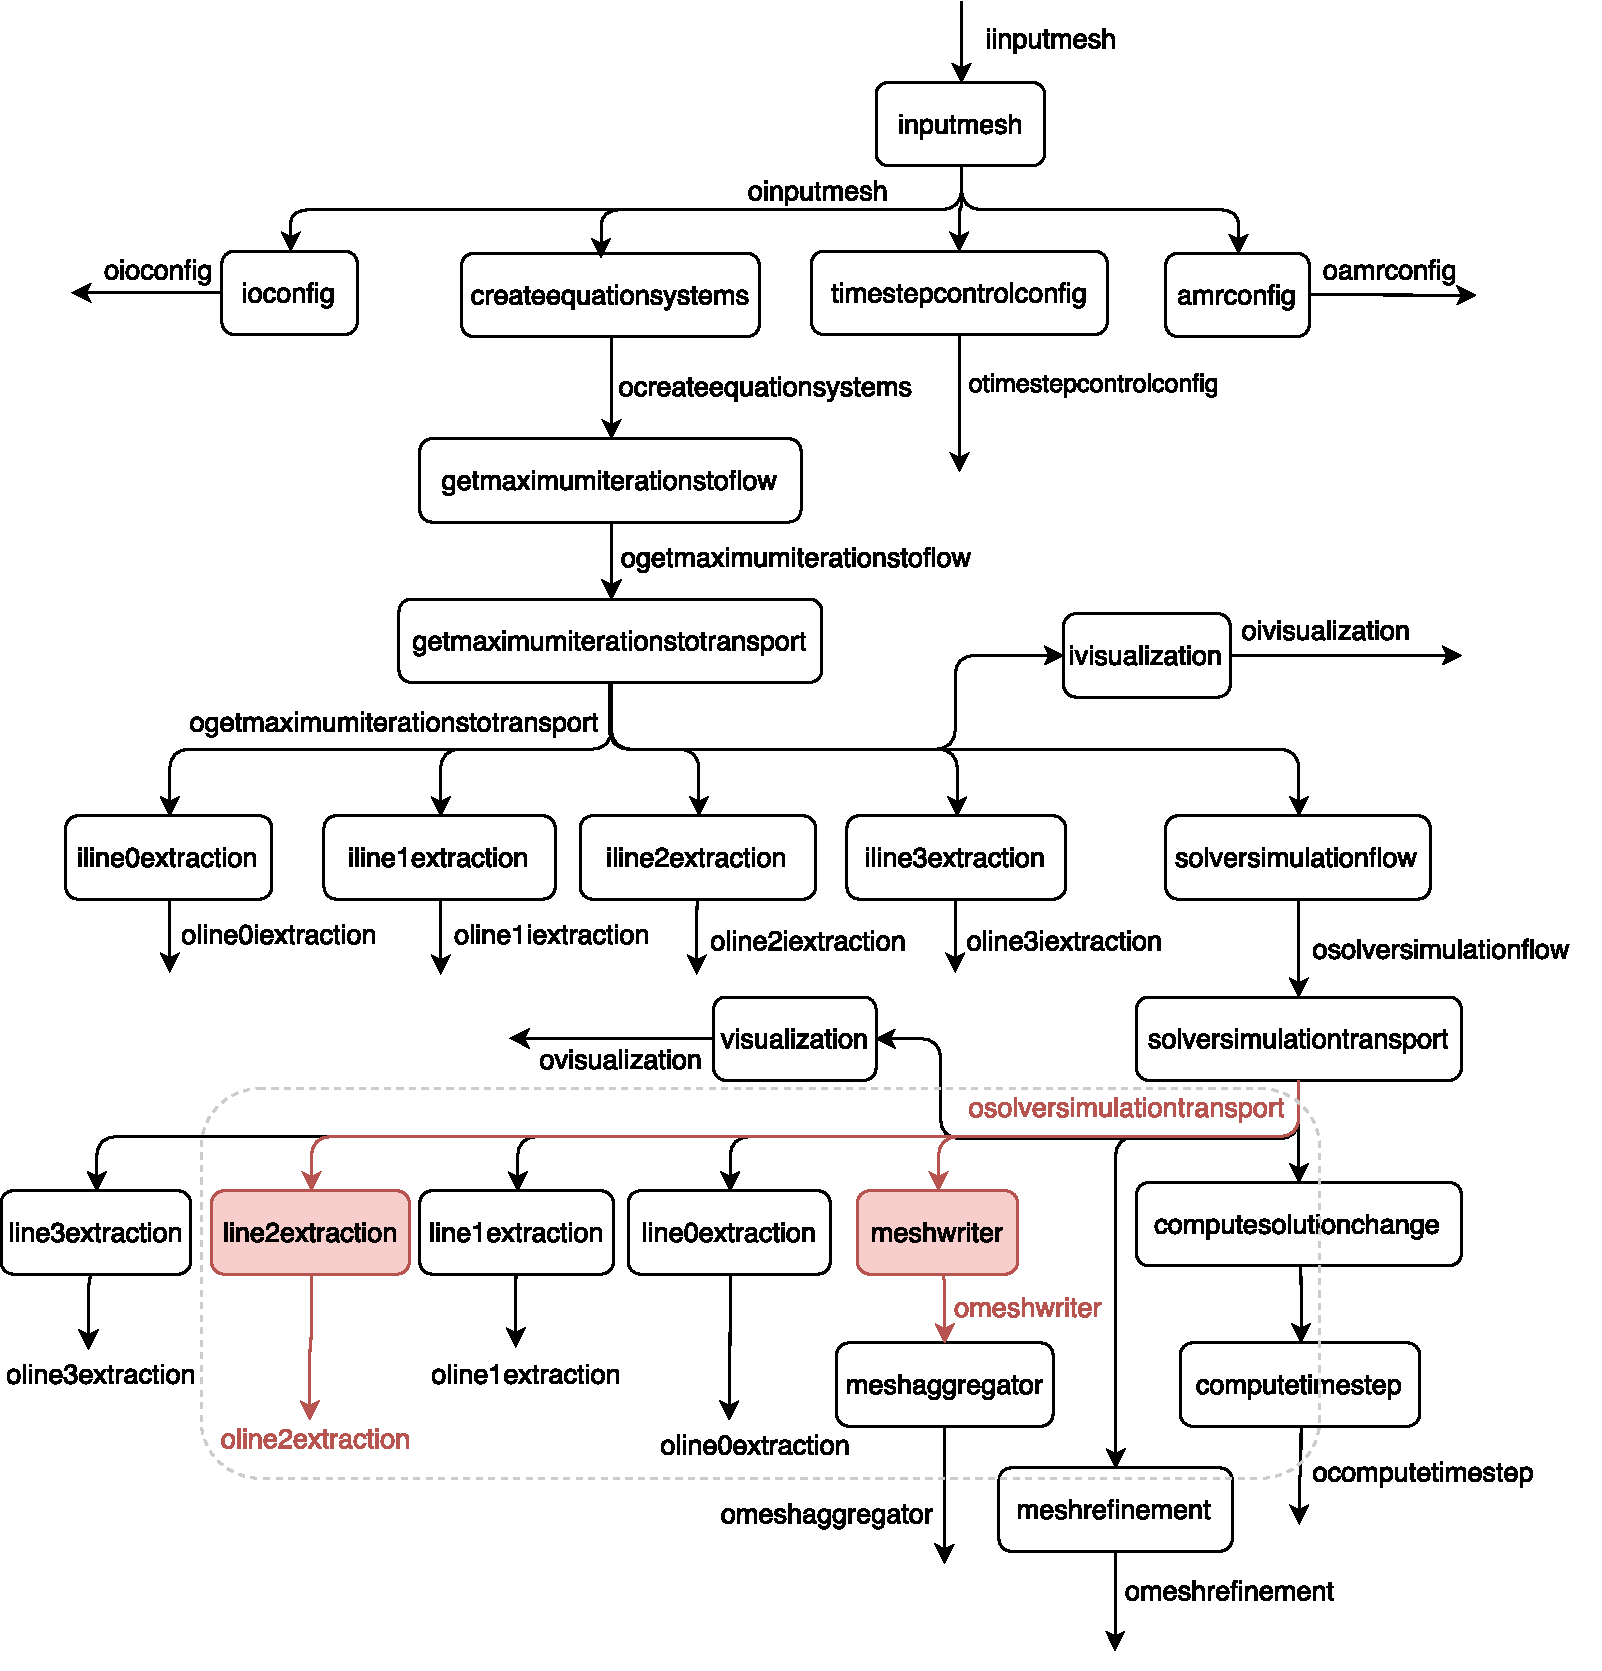
\includegraphics[width=\textwidth]{img/experiments-dataflow-1}
    \caption[Caminho do fluxo de dados \(D^{\dagger}\) rastreado na consulta \#1]{Caminho d fluxo de dados \(D^{\dagger}\) rastreado na consulta \#1.}%
    \label{fig:experiments-dataflow-1}
\end{figure}

\begin{minipage}[c]{0.95\textwidth}
\begin{lstlisting}[language=sql,label={lst:experiments-1-sql},caption={[Código em SQL gerado na consulta~\#1]Código em SQL gerado na consulta~\#1 (40,29~ms).}]
SELECT osolversimulationtransport.time, AVG(oline2extraction.d)
FROM osolversimulationtransport, oline2extraction, omeshwriter
WHERE (osolversimulationtransport.line2extraction_task_id = oline2extraction.line2extraction_task_id) 
AND (osolversimulationtransport.meshwriter_task_id = omeshwriter.meshwriter_task_id)
GROUP BY osolversimulationtransport.time;
\end{lstlisting}
\end{minipage}

\begin{minipage}[c]{0.95\textwidth}
\begin{lstlisting}[language=sqlresults,label={lst:experiments-1-sqlresults},caption={[Resultados da consulta \#1.]Resultados da consulta \#1 (7 tuplas, 4,346~ms).}]
+--------------------------+--------------------------+
| time                     | L71                      |
+==========================+==========================+
|                1.3398483 |     1.74129306930693e-44 |
|                3.1009347 |  -1.0847045643564339e-44 |
|                5.4124618 |    7.853749801980205e-39 |
|                7.8695609 |  -1.8180726336633645e-33 |
|               10.1307669 |   1.0729463267326738e-27 |
|               12.6055519 |   1.0473414950495052e-24 |
|                       15 |   -8.768540693069305e-22 |
+--------------------------+--------------------------+
\end{lstlisting}
\end{minipage}

\subsection{Consulta \#2}

\perrotta{TODO: observação: LIMIT 10}

\begin{table}[htb]
    \centering
    \begin{tabular}{c|c}
\textbf{Argumento}          & \textbf{Valor} \\ \hline
\texttt{D}                  & $D^{\dagger}$ \\
\texttt{dsOrigins}          & \{\texttt{osolversimulationtransport}\} \\
\texttt{dsDestinations}     & \{\texttt{oline0extraction}, \texttt{omeshwriter}\} \\
\texttt{type}               & physical \\ \hline
\texttt{projections}        & \makecell{\{\texttt{osolversimulationtransport.time}, \\
                                          \texttt{oline0extraction.points0}, \\ 
                                          \texttt{oline0extraction.points1}, \texttt{oline0extraction.points2}, \\
                                          \texttt{oline0extraction.d}\}} \\ \hline
\texttt{selections}         & \makecell{\{\texttt{osolversimulationtransport.time < 5.5}, \\
                                          \texttt{oline0extraction.d > 0.1}\}} \\ \hline
\texttt{dsIncludes}         & \varnothing \\
\texttt{dsExcludes}         & \varnothing \\
    \end{tabular}
    \caption[Argumentos da função \texttt{generateSqlQuery} para a consulta \#2]{Especificação dos argumentos da função \texttt{generateSqlQuery} para a consulta~\#2.}%
    \label{tab:experiments-2-especificacao}
\end{table}

\begin{figure}[htb]
    \centering
    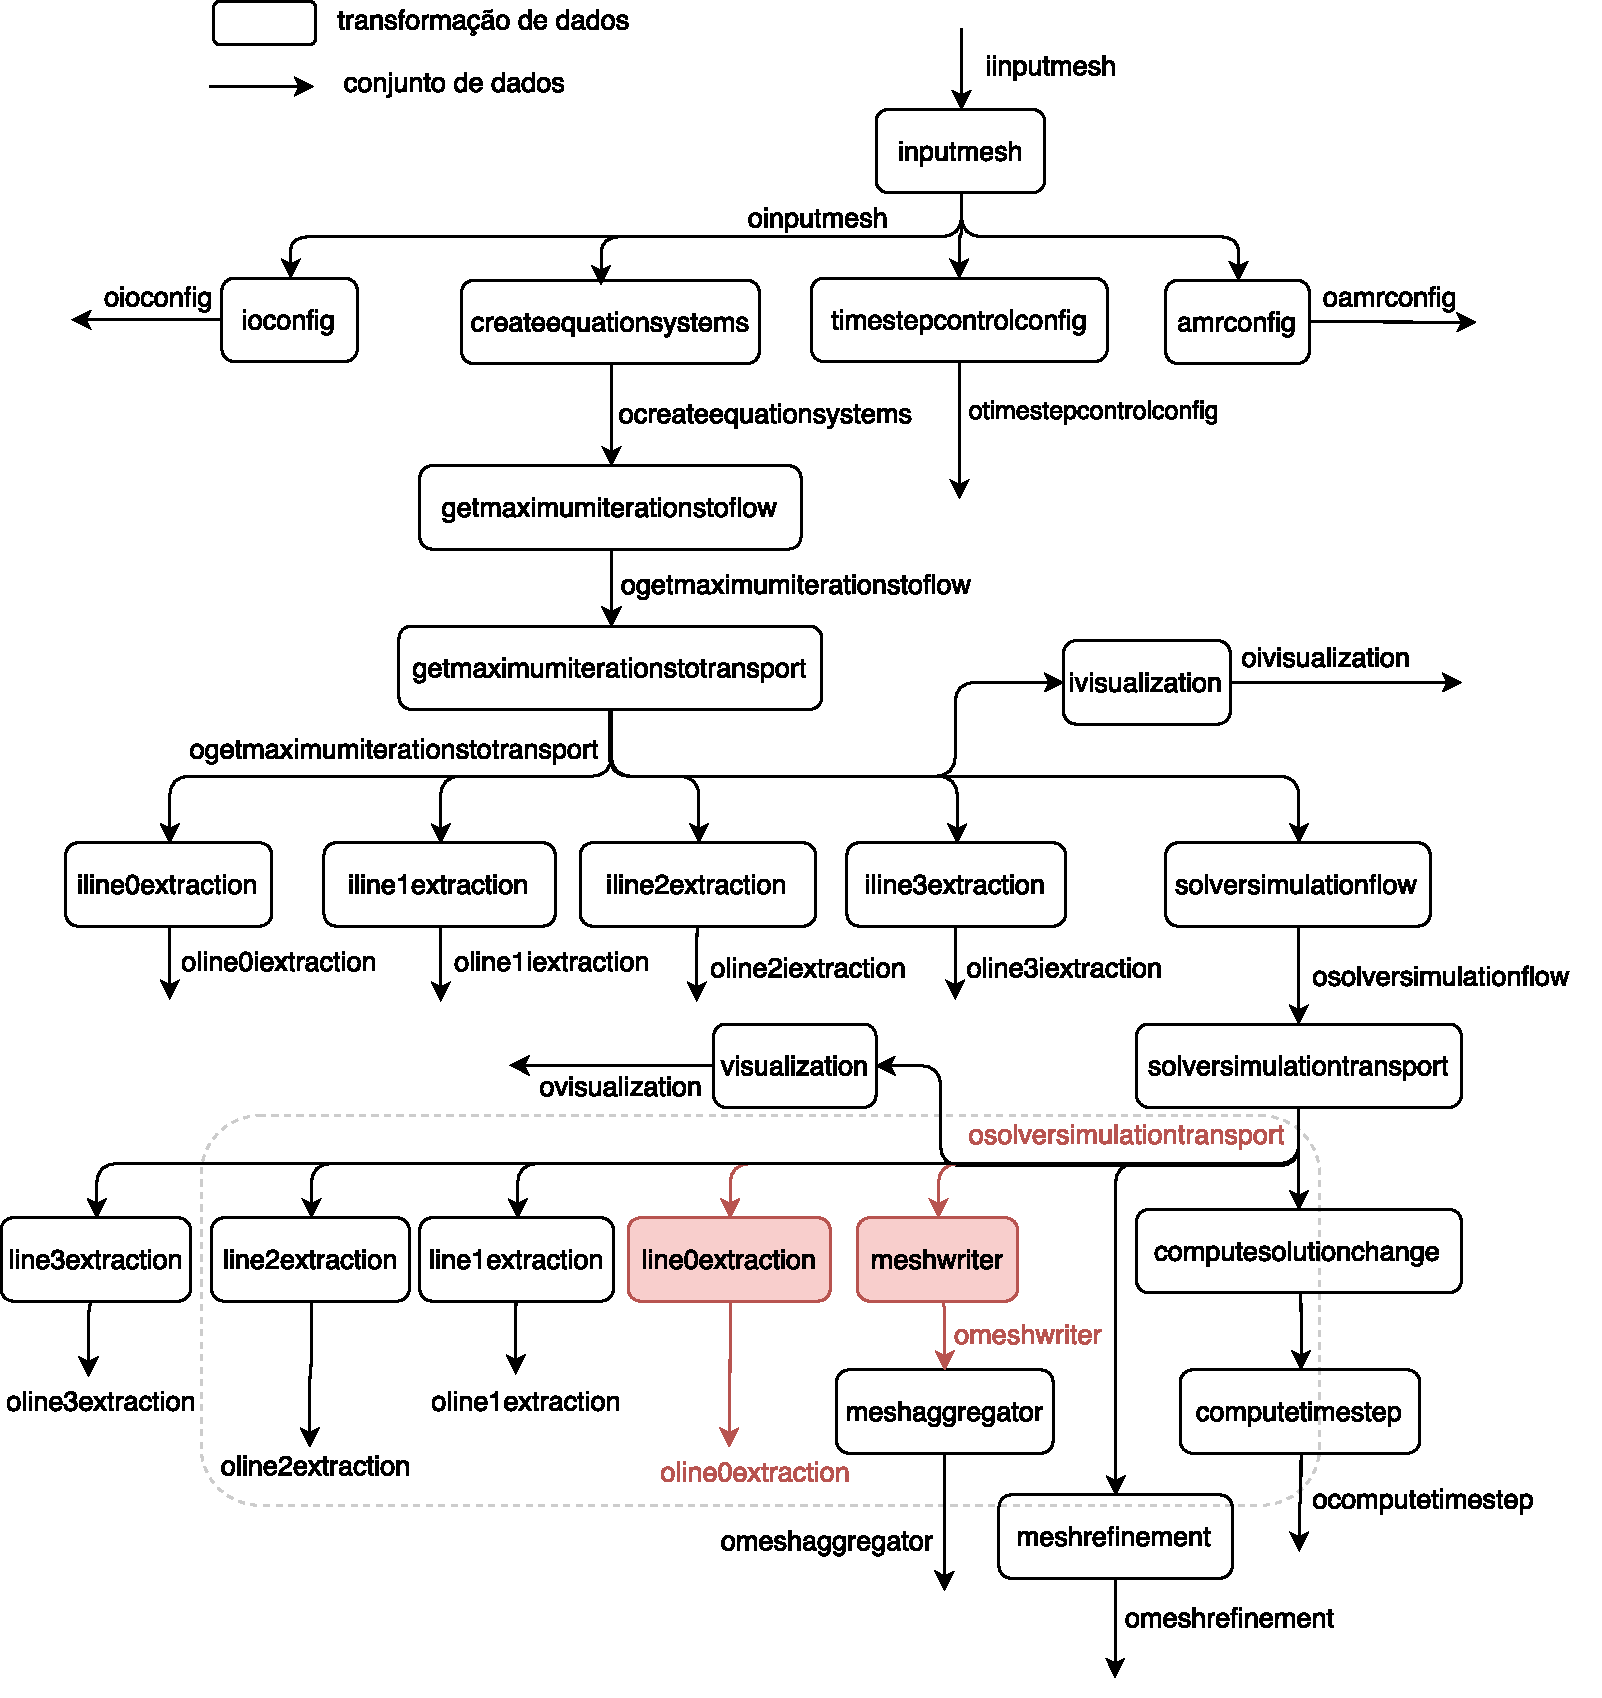
\includegraphics[width=\textwidth]{img/experiments-dataflow-2}
    \caption[Caminho do fluxo de dados \(D^{\dagger}\) rastreado na consulta \#2]{Caminho d fluxo de dados \(D^{\dagger}\) rastreado na consulta \#2.}%
    \label{fig:experiments-dataflow-2}
\end{figure}

\begin{minipage}[c]{0.95\textwidth}
\begin{lstlisting}[language=sql,label={lst:experiments-2-sql},caption={[Código em SQL gerado na consulta~\#2]Código em SQL gerado na consulta~\#2 (15,45~ms).}]
SELECT osolversimulationtransport.time, oline0extraction.points0, oline0extraction.points1, oline0extraction.points2, oline0extraction.d
FROM osolversimulationtransport, oline0extraction, omeshwriter
WHERE (osolversimulationtransport.time < 5.5) 
AND (oline0extraction.d > 0.1) 
AND (osolversimulationtransport.line0extraction_task_id = oline0extraction.line0extraction_task_id) 
AND (osolversimulationtransport.meshwriter_task_id = omeshwriter.meshwriter_task_id)
LIMIT 10;
\end{lstlisting}
\end{minipage}

\begin{minipage}[c]{0.95\textwidth}
\begin{lstlisting}[language=sqlresults,label={lst:experiments-2-sqlresults},caption={[Resultados da consulta \#2.]Resultados da consulta \#2 (10 tuplas, 5,92~ms).}]
+--------------+-----------+---------+---------+----------+
| time         | points0   | points1 | points2 | d        |
+==============+===========+=========+=========+==========+
|    5.4124618 |         0 |       1 |       0 |  0.10814 |
|    5.4124618 |      0.18 |       1 |       0 |   0.1082 |
|    5.4124618 |      0.36 |       1 |       0 |  0.10825 |
|    5.4124618 |      0.54 |       1 |       0 |  0.10825 |
|    5.4124618 |      0.72 |       1 |       0 |  0.10825 |
|    5.4124618 |         0 |       1 |       0 |  0.10814 |
|    5.4124618 |      0.18 |       1 |       0 |   0.1082 |
|    5.4124618 |      0.36 |       1 |       0 |  0.10825 |
|    5.4124618 |      0.54 |       1 |       0 |  0.10825 |
|    5.4124618 |      0.72 |       1 |       0 |  0.10825 |
+--------------+-----------+---------+---------+----------+
\end{lstlisting}
\end{minipage}

% |    5.4124618 |         0 |       1 |       0 |  0.10814 |
% |    5.4124618 |      0.18 |       1 |       0 |   0.1082 |
% |    5.4124618 |      0.36 |       1 |       0 |  0.10825 |
% |    5.4124618 |      0.54 |       1 |       0 |  0.10825 |
% |    5.4124618 |      0.72 |       1 |       0 |  0.10825 |
% |    5.4124618 |         0 |       1 |       0 |  0.10814 |
% |    5.4124618 |      0.18 |       1 |       0 |   0.1082 |
% |    5.4124618 |      0.36 |       1 |       0 |  0.10825 |
% |    5.4124618 |      0.54 |       1 |       0 |  0.10825 |
% |    5.4124618 |      0.72 |       1 |       0 |  0.10825 |

\subsection{Consulta \#3}

\perrotta{TODO: consulta \#3}

\subsection{Consulta \#4}

\perrotta{TODO: consulta \#4}
  % !TEX encoding = UTF-8 Unicode
% -*- coding: UTF-8; -*-
% vim: set fenc=utf-8

\chapter{Conclusão}%
\label{chap:conclusao}

\section{Considerações Finais}

Nesta monografia foi proposto o \textbf{QPP (Pré-Processador de Consultas)} como componente integrante ao DfAnalyzer, instanciando a arquitetura ARMFUL~\cite{silva2017raw} para a análise de simulações computacionais e fluxo de dados em larga escala. Para isso, os conceitos de fluxo de dados e mapeamento de atributos de dados comumente utilizados em consultas a simulações computacionais, assim como os tipos de proveniência prospectiva e retrospectiva foram revisitados a fim de propor a nossa abordagem para análise de dados de simulação. Mais especificamente, nossa abordagem baseou-se no conceito de rastro de dados de proveniência tirando proveito dos mapeamentos físicos e lógicos de atributos na especificação do fluxo de dados em simulações computacionais. 

Por meio da função \texttt{generateSqlQuery}, o QPP pode potencialmente facilitar a interação dos usuários com o sistema ao analisar dados de proveniência, de execução e de domínio armazenados na base de dados do DfAnalyzer~\cite{gadelha2012mtcprov}. Por exemplo, operações de junção comumente necessárias para relacionar conjuntos de dados oriundos da simulação não precisam ser especificadas explicitamente ao realizar análises usando o QPP. Assim, os usuários não precisam compreender todos os relacionamentos presentes no esquema da base de dados para realizar as suas consultas, diminuindo, assim, a curva de aprendizado e o esforço necessário da parte do usuário envolvidos na análise exploratória de dados científicos, uma vez que os principais relacionamentos entre conjuntos de dados são representados através de mapeamentos de atributos de dados do tipo lógico. Tais atributos de dados são devidamente levados em consideração na geração do código em SQL a partir do grafo de junção do fluxo de dados, o que seria complexo e trabalhoso se fosse realizado direta e manualmente pelo usuário.
Além disso, uma vez que os dados de proveniência são organizados em um DAG, a realização de consultas no modelo relacional para percorrer esse grafo também é um fator de complexidade adicional, o qual é abstraído para o usuário através do QPP.
No \autoref{chap:experimentos}, diversas consultas relacionadas a uma aplicação real~\cite{silva2016situ} foram executadas, ilustrando a utilização do QPP e o seu potencial analítico, e demonstrando a adequação e a eficiência da solução proposta.

\section{Trabalhos Futuros}

Dentre algumas ideias de trabalhos futuros para o projeto do pré-processador de consultas, destacam-se:

\begin{itemize}
    % Projeto da Débora: visualizador
    \item a implementação e integração de uma \textbf{interface gráfica} para o pré-processador de consultas, com o intuito e potencial de melhorar a usabilidade para o usuário e, mais especificamente: (\(i\)) auxiliá-lo a criar e especificar consultas, através da ação de arrastar e soltar com o \textit{mouse} etiquetas com as transformações e conjuntos de dados; e (\(ii\)) apresentá-lo os resultados da execução da consulta em SQL no banco de dados de forma visualmente organizada e limpa.
    % Otimizações de consultas que discutimos.
    \item aumentar o \textbf{desempenho das consultas} em SQL, com uma (\(i\)) diminuição do \textit{overhead} do pré-processador de consultas, através do aumento do desempenho da conversão das especificações do usuário para a linguagem SQL; e da (\(ii\)) otimização da consulta em si, por exemplo, através de melhorias nas técnicas de indexação, ou da diminuição do número de projeções e~/~ou junções incluídas na mesma, ou mesmo via um melhor aproveitamento das informações e dados de proveniência disponíveis no banco de dados.
    \item implementar uma forma de \textbf{validação nas especificações do usuário}, permitindo apenas a geração de consultas sintática e semanticamente válidas, com o intuito de melhorar o \textit{design} de interação e diminuir a probabilidade de erros por parte do mesmo, \textit{e.g.}, permitir apenas conjuntos de dados existentes nas projeções especificadas pelo usuário.
    \item permitir a inclusão de subconsultas na consulta principal e adicionar suporte a mais cláusulas da linguagem SQL, a fim de suportar consultas mais complexas: por exemplo, \texttt{GROUP BY}, \texttt{SELECT DISTINCT} e \texttt{LIMIT}.
    \item validar a hipótese de que o QPP realmente auxilia e facilita a interação de usuários reais com o sistema apresentado, checando se a curva de aprendizado para realizar consultas em simulações computacionais, com a utilização do QPP, realmente diminui.
\end{itemize}
 % Conclusion

  \backmatter{}
  \appendix
  % !TEX encoding = UTF-8 Unicode
% -*- coding: UTF-8; -*-
% vim: set fenc=utf-8

\chapter{Funções auxiliares}%
\label{app:funcoes-auxiliares}

Nesse capítulo são listadas as funções auxiliares referenciadas e utilizadas nos algoritmos da \autoref{sec:algoritmos-utilizados}, na ordem de aparecimento neste documento.

\begin{lstlisting}[language=pseudocode,label={lst:get-next-transformations},caption={[Obtenção das próximas transformações de dados de uma transformação]Obtenção das próximas transformações de dados de uma transformação de dados.}]
function getNextTransformations(D, dt):
    transformations %\leftarrow% {}
    for each %\phi% %\in% %D.\Phi% do:
        if %$\phi.dt_{\textup{previous}}$% = dt and %$\phi.dt_{\textup{next}}$% %\ne% %\varnothing% then:
            transformations %\leftarrow% transformations + 
        end if
    end do
    return transformations
end function
\end{lstlisting}
 \begin{lstlisting}[language=pseudocode,label={lst:has-many-output-datasets},caption={[Contagem dos conjuntos de dados de saída de uma transformação]Contagem dos conjuntos de dados de saída de uma transformação de dados. Retorna verdadeiro caso essa quantidade seja maior do que um, e falso caso contrário.}]
function hasManyOutputDatasets(D, dt):
    count %\leftarrow% 0
    for each %\phi% %\in% %D.\Phi% do:
        if %$\phi.dt_{\textup{previous}}$% = dt and %$\phi.ds$% %\ne% %\varnothing% then:
            count %\leftarrow% count + 1
            if count > 1 then:
                return true
            end if
        end if
    end do
    return false
end function
\end{lstlisting}
 \begin{lstlisting}[language=pseudocode,label={lst:has-many-next-transformations},caption={[Contagem das próximas transformações de dados de uma transformação]Contagem das próximas transformações de dados de uma transformação de dados. Retorna verdadeiro caso essa quantidade seja maior do que um, e falso caso contrário.}]
function hasManyNextTransformations(D, dt):
    count %\leftarrow% 0
    for each %\phi% %\in% %D.\Phi% do:
        if %$\phi.dt_{\textup{previous}}$% = dt and %$\phi.dt_{\textup{next}}$% %\ne% %\varnothing% then:
            count %\leftarrow% count + 1
            if count > 1 then:
                return true
            end if
        end if
    end do
    return false
end function
\end{lstlisting}
 \begin{lstlisting}[language=pseudocode,label={lst:any-transformation-has-many-input-datasets},caption={[Determinação de se pelo menos uma transformação possui mais de um conjunto de dados de entrada.]Determinação de se pelo menos uma transformação de dados possui mais de um conjunto de dados de entrada. Retorna verdadeiro caso positivo, e falso caso contrário.}]
function anyTransformationHasManyInputDatasets(D, dts):
    for each dt %\in% dts do:
        if hasManyInputDatasets(D, dt) then:%~\quad%#%~\autoref{lst:has-many-input-datasets}%
            return true
        end if
    end do
    return false
end function
\end{lstlisting}
 \begin{lstlisting}[language=pseudocode,label={lst:has-many-input-datasets},caption={[Contagem dos conjuntos de dados anteriores a uma transformação]Contagem dos conjuntos de dados anteriores a uma transformação de dados. Retorna verdadeiro caso essa quantidade seja maior do que um, e falso caso contrário.}]
function hasManyInputDatasets(D, dt):
    count %\leftarrow% 0
    for each %\phi% %\in% %D.\Phi% do:
        if %$\phi.dt_{\textup{next}}$% = dt and %$\phi.ds$% %\ne% %\varnothing% then:
            count %\leftarrow% count + 1
            if count > 1 then:
                return true
            end if
        end if
    end do
    return false
end function
\end{lstlisting}
 \begin{lstlisting}[language=pseudocode,label={lst:get-transformation-track},caption={[Obtenção da trilha de transformações de uma transformação.]Obtenção da trilha de transformações de uma transformação.}]
function getTransformationTrack(dtTracks,dt):
    for dtTrack %\in% dtTracks:
        if dt %\in% dtTrack then:
            return dtTrack
        end if
    end do
    return %\varnothing%
end function
\end{lstlisting}

\begin{lstlisting}[language=pseudocode,label={lst:get-previous-transformations},caption={[Obtenção das transformações de dados anteriores a uma transformação]Obtenção das transformações de dados anteriores a uma transformação de dados.}]
function getPreviousTransformations(D, dt):
    transformations %\leftarrow% {}
    for each %\phi% %\in% %D.\Phi% do:
        if %$\phi.dt_{\textup{next}}$% = dt and %$\phi.dt_{\textup{previous}}$% %\ne% %\varnothing% then:
            transformations %\leftarrow% transformations + 
        end if
    end do
    return transformations
end function
\end{lstlisting}

\begin{lstlisting}[language=pseudocode,label={lst:get-next-datasets},caption={[Obtenção dos próximos conjuntos de dados de uma transformação]Obtenção dos próximos conjuntos de dados de uma transformação de dados.}]
function getNextDatasets(D, dt):
    datasets %\leftarrow% {}
    for each %\phi% %\in% %D.\Phi% do:
        if %$\phi.dt_{\textup{previous}}$% = dt and %\phi.ds% %\ne% %\varnothing% then:
            datasets %\leftarrow% datasets + 
        end if
    end do
    return datasets
end function
\end{lstlisting}

\begin{lstlisting}[language=pseudocode,label={lst:get-previous-datasets},caption={[Obtenção dos conjuntos de dados anteriores a uma transformação]Obtenção dos conjuntos de dados anteriores a uma transformação de dados.}]
function getPreviousDatasets(D, dt):
    datasets %\leftarrow% {}
    for each %\phi% %\in% %D.\Phi% do:
        if %$\phi.dt_{\textup{next}}$% = dt and %\phi.ds% %\ne% %\varnothing% then:
            datasets %\leftarrow% datasets + 
        end if
    end do
    return datasets
end function
\end{lstlisting}

\begin{lstlisting}[language=pseudocode,label={lst:get-next-datasets-2},caption={[Obtenção dos próximos conjuntos de dados de um conjunto de dados]Obtenção dos próximos conjuntos de dados de um conjunto de dados.}]
function getNextDatasets(D, ds):
    datasets %\leftarrow% {}
    for each %\phi% %\in% %D.\Phi% do:
        if %$\phi.ds$% = ds:
            datasets %\leftarrow% datasets + {getNextDatasets(%$\phi.dt_{\textup{next}}$%)}%~\quad%#%~\autoref{lst:get-next-datasets}%
        end if
    end do
    return datasets
end function
\end{lstlisting}

\begin{lstlisting}[language=pseudocode,label={lst:get-transformation},caption={[Obtenção da transformação entre dois conjuntos de dados]Obtenção da transformação de dados associada a dois conjuntos de dados.}]
function getTransformation(D, %$ds_1$%, %$ds_2$%):
    for each %\phi% %\in% %D.\Phi% do:
        if %$\phi.ds$% = %$ds_1$% and %$ds_2$% %\in% getNextDatasets(%$\phi.dt_{\textup{next}}$%) then:%~\quad%#%~\autoref{lst:get-next-datasets}%
            return %$\phi.dt_{\textup{next}}$%
        else if %$\phi.ds$% = %$ds_2$% and %$ds_1$% %\in% getNextDatasets(%$\phi.dt_{\textup{next}}$%) then:%~\quad%#%~\autoref{lst:get-next-datasets}%
            return %$\phi.dt_{\textup{next}}$%
        end if
    end do
    return %\varnothing%
end function
\end{lstlisting}
  
  \bibliographystyle{coppetex/coppe-unsrt}
  \bibliography{thesis} % Pro-Tip: use JabRef to manage this file

\end{document}